\documentclass[a4paper,12pt]{report}
\usepackage[francais]{babel}
\usepackage{graphicx}
\usepackage{lipsum}
\usepackage{amsmath,amsfonts,amssymb}
\usepackage[T1]{fontenc}
\usepackage[utf8]{inputenc}

\usepackage{array}
\usepackage{afterpage}

\usepackage{geometry}
\geometry{top=3cm, bottom=3cm, left=2.5cm, right=2.5cm}

\usepackage{hyperref}
\usepackage{framed}

\usepackage{rotating}
\usepackage{caption}

\usepackage{fancyhdr}
\setlength{\headheight}{15.2pt}
%\pagestyle{fancy}
%\lhead[]{Left header}
%\rhead[]{Right header}
\pagestyle{fancy}
\fancyhead[L]{ \bfseries\nouppercase{\rightmark} }
\fancyhead[R]{\bfseries \thepage}
\fancyfoot[LCR]{}



\newcommand{\bi}{\begin{itemize}}
\newcommand{\ei}{\end{itemize}}
\newcommand{\itemo}{\item[\textsf{o}]}

\graphicspath{{./images/}}

\begin{document}


\begin{titlepage}
\begin{center}

\includegraphics[width=7cm]{images/logo.png}\\[1cm]
{\Large Projet Ingénierie et Entrepreneuriat}\\[0.5cm]
{\Large Projet 86}\\[0.5cm]
% Title
\rule{\linewidth}{0.5mm} \\[0.4cm]
{ \huge \bfseries Génération rapide de trajectoire pour voiture autonome \\[0.4cm] }
\rule{\linewidth}{0.5mm} \\[1.5cm]
% Author and supervisor
\noindent

\begin{center} \large
	Étudiants : \\
	\vspace*{0.3cm}
	Médéric \textsc{Fourmy}\\
	William \textsc{Jussiau}\\
        Guillermo \textsc{Prieto}\\
        Martin \textsc{Renou}\\
        Jan \textsc{Zeman}\\
\end{center}

\vspace*{1cm}

\begin{center} \large
	Tutrice en gestion de projet : \\
	Frédérique \textsc{Martin}, {AIRBUS} \\
	
		\vspace*{0.5cm}

	Responsable technique : \\
	Diane \textsc{Bury}, {CNRS-LAAS} \\
	
		\vspace*{0.5cm}

	Client : \\
	Nicolas \textsc{Mansard}, {CNRS-LAAS}
\end{center}

\vfill
\end{center}
\end{titlepage}








%%%%%%%%%%%%%%%%%%%%%%%%%%%%%%%%%%%%%%%%%%%%%%%%%%%%%%%%%
\pagebreak
\afterpage{\null\newpage}
\clearpage

\renewcommand{\abstractname}{Résumé}

\begin{abstract}

\noindent\hrulefill


Ce document présente le travail effectué pendant l'année scolaire 2017-2018 dans le cadre du PIE \og Génération rapide de trajectoire pour voiture autonome, sous l'encadrement de deux tuteurs du CNRS-LAAS et d'une tutrice en gestion de projet, d'Airbus.

Le projet a consisté à s'intéresser à une approche développée au LAAS pour la génération rapide de trajectoire, basée sur l'interaction entre un réseau de neurones et un algorithme de contrôle prédictif.

Afin de démontrer la pertinence d'un tel algorithme et son intérêt par rapport à la méthode traditionnelle de contrôle prédictif, nous avons développé un simulateur de voiture autonome exploitant cette méthode. Celui-ci se base sur l'utilisation des logiciels ROS et Gazebo, classiques dans le domaine de la robotique.


\vspace*{1cm}

\textbf{Mots-clés :} voiture autonome, simulateur, contrôle prédictif, réseau de neurones, IREPA, ROS, Gazebo, CNRS-LAAS


\noindent\hrulefill

\end{abstract}



%\noindent\hrulefill
%\vfill
%\hspace{0pt}
%%%%%%%%%%%%%%%%%%%%%%%%%%%%%%%%%%%%%%%%%%%%%%%%%%%%%%%%%



%%%%%%%%%%%%%%%%%%%%%%%%%%%%%%%%%%%%%%%%%%%%%%%%%%%%%%%%%


\renewcommand{\abstractname}{Déclaration d'authenticité}
\begin{abstract}
Nous déclarons solennellement que le travail présenté a été produit entièrement par notre équipe d'étudiants pendant l'année scolaire 2017-2018. 

Dans le cas de l'utilisation de ressources extérieures, celles-ci seront dûment citées et leurs auteurs remerciés.

\end{abstract}


%\vfill
%\hspace{0pt}
%\addcontentsline{toc}{section}{Déclaration d'authenticité}
%%%%%%%%%%%%%%%%%%%%%%%%%%%%%%%%%%%%%%%%%%%%%%%%%%%%%%%%%




%%%%%%%%%%%%%%%%%%%%%%%%%%%%%%%%%%%%%%%%%%%%%%%%%%%%%%%%%
\tableofcontents
%%%%%%%%%%%%%%%%%%%%%%%%%%%%%%%%%%%%%%%%%%%%%%%%%%%%%%%%%

















%%%%%%%%%%%%%%%%%%%%%%%%%%%%%%%%%%%%%%%%%%%%%%%%%%%%%%%%%
\newpage
\chapter*{Introduction}
\addcontentsline{toc}{chapter}{Introduction}

\subsection*{Le contexte}
Avec le développement récent de voitures dites autonomes dont l'accessibilité au grand public est prédite pour les années 2020 \cite{autonomous_car}\cite{autonomous_car_2}, les thématiques liées au pilotage de ces engins sont devenues très actuelles. Le CNRS-LAAS \cite{laas}, acteur incontournable de la recherche en robotique en France, a dans ce contexte mandaté un projet sur la génération rapide de trajectoire pour un véhicule autonome en partenariat avec l'ISAE-SUPAERO. Ce projet prend la forme d'un Projet Ingénierie et Entrepreneuriat (PIE) proposé à une équipe de 5 étudiants de troisième année, encadrés par deux chercheurs du LAAS et une tutrice en gestion de projet, d'Airbus.


\subsection*{Le projet}
Le projet fait suite à un projet réalisé l'année dernière, dans lequel les étudiants ont appliqué des techniques de commande prédictive à un drone quadrirotor. L'un des problèmes majeurs de cette approche est que le contrôleur de bord doit recalculer entièrement la trajectoire à une fréquence donnée, opération gourmande en temps et en énergie. Ici, on s'intéressera à l'implémentation d’un algorithme développé au LAAS qui améliore l’approche précédente : un pré-calcul hors-ligne détermine de bonnes trajectoires et les stocke dans un réseau de neurones. Celui-ci, embarqué sur le système réel, donne une bonne première approximation de la trajectoire en temps réel (et avec un faible coût calculatoire), qui est ensuite raffinée par un contrôleur prédictif. Notre travail se base sur une publication scientifique issue du LAAS où l'algorithme IREPA (pour \textit{Iterative Roadmap Extension and Policy Approximation}) et son utilisation sont expliquées plus en détails \cite{mansard}.

L'objectif du projet est de développer pour le LAAS un démonstrateur de voiture autonome exploitant cette approche, afin de mettre en avant sa pertinence par rapport au contrôle prédictif traditionnel. Nous avons choisi de nous baser sur l'utilisation du logiciel de communication ROS \cite{ROS} et du simulateur Gazebo \cite{Gazebo}, deux références en robotique.

\subsection*{Ce document}
Ce rapport se décompose en trois parties. Dans une première, on abordera la façon dont le projet a été géré : méthodes de travail, répartition des tâches et des responsabilités, conventions, définition de jalons... Dans une seconde partie, on détaillera la manière dont on a réalisé le projet : architecture, logiciels utilisés, code, méthodes employées... Enfin, dans une dernière partie, on mettra en avant notre contribution et on donnera quelques pistes pour une éventuelle suite.

%%%%%%%%%%%%%%%%%%%%%%%%%%%%%%%%%%%%%%%%%%%%%%%%%%%%%%%%%








%%%%%%%%%%%%%%%%%%%%%%%%%%%%%%%%%%%%%%%%%%%%%%%%%%%%%%%%%
\chapter{Gestion de projet}

\section{Description du projet}
\subsection{Objectifs, périmètre}

\subsubsection{Objectif} 
L'objectif de ce projet est unique et a été bien défini au départ par le mandataire du projet. Il s'agit de :

\begin{center}
\textit{Prouver, en développant un démonstrateur, la pertinence de la méthode de génération rapide de trajectoire basée sur l'approche \cite{mansard} dans le cas de la voiture autonome}.
\end{center}


\subsubsection{Périmètre} 
Le périmètre du projet a été contraint de sorte que l'objectif reste réalisable dans le temps imparti. En particulier, certaines des limites du simulateur sont les suivantes :
\bi
\itemo la voiture connaît parfaitement son environnement : on considère que la chaîne de perception (traitement d'images, de données radar/lidar, etc.) qui existerait sur un système réel nous fournit toutes les informations nécessaires et exemptes de bruit de mesure,
\itemo le modèle et les paramètres de la voiture sont supposés entièrement connus et déterministes,
\itemo les calculs seront effectués et leurs performances seront évaluées sur une architecture de calcul classique (non embarquée, ex. processeur Intel i7, exécution du code à 10 Hz). Cela ne devra pas empêcher le portage sur un calculateur embarqué,
\itemo la voiture ne sera pas manipulée en temps réel par un utilisateur disposant d'un clavier ou d'un joystick. Les paramètres de l'environnement (obstacles) et de la trajectoire (départ, arrivée) seront choisis par l'utilisateur avant la simulation.
\ei



\subsubsection{Exigences fonctionnelles} 
En l'absence de spécifications fonctionnelles précises sur la forme, nous avons pu décider (avec accord du client) quelques contraintes haut niveau, qui sont les suivantes :
\begin{enumerate}
\item le démonstrateur devra être facile à lancer et à manipuler pour un utilisateur sans connaissance préalable,
\item le code devra être le plus modulaire et réutilisable possible, afin de favoriser une éventuelle extension du projet.
\end{enumerate}

\bigskip

Quelques exigences, énoncées implicitement dans la description du projet, sont aussi détaillées ci-dessous :
\begin{itemize}

\itemo Documentation : le démonstrateur doit posséder une documentation technique, qui comprend :
	\bi
	\item une procédure explicative d'installation,
	\item une liste exhaustive des ressources externes nécessaires,
	\item un manuel d'instructions pour l'utilisation du logiciel.
	\ei
	
\itemo Démonstrateur : le démonstrateur doit respecter les exigences suivantes :
	\bi
	\item simuler une voiture dans le cas nominal,
	\item simuler et représenter un environnement contenant des obstacles,
	\item opérer sous un environnement Linux,
	\item s'exécuter en temps réel,
	\item ses ressources externes (ex. librairies, logiciels) doivent être bien identifiées et répertoriées.
	\ei
	
\itemo Algorithme : la génération rapide de trajectoire devra respecter certaines règles :
	\bi
	\item l'algorithme se base sur l'article cosigné par notre tuteur Nicolas Mansard :  "Using a memory of motion to efficiently warm-start a nonlinear predictive controller" \cite{mansard}. Par abus de langage, dans la suite du rapport, on pourra désigner la méthode décrite dans cette article par le sigle IREPA (qui correspond en fait à la partie apprentissage de l'estimateur),
	\item l'algorithme doit permettre de générer une trajectoire entre deux points du plan,
	\item l'algorithme doit empêcher toute collision avec un obstacle.
	\ei

\itemo Interface utilisateur : le logiciel disposera d'une interface utilisateur basique respectant les contraintes :
	\bi
	\item l'utilisateur doit pouvoir choisir les points de départ et d'arrivée de la trajectoire,
	\ei
	
\end{itemize}


\bigskip

\subsubsection{Contraintes :}

Le contexte dans lequel s'inscrit le projet a pour conséquence l'apparition de quelques contraintes que nous devrons prendre en compte dans le développement, à savoir :

\bi
\itemo Développement logiciel : 

	\bi
	\item Utilisation de logiciels et librairies : le projet devra s'inscrire dans une continuité relative avec le projet de l'année dernière sur le drone quadrirotor. Ainsi, il nous devrons utiliser l'outil de gestion de sources Git/GitHub pour la collaboration, ainsi que la librairie de calcul ACADO \cite{acado} pour le contrôle prédictif,
	
	\item Philosophie de développement : dans un souci d'universalité, nous nous imposerons des normes de codage (GNU Coding Standards \cite{gnu} pour C et bash, PEP8 \cite{pep8} pour Python).
		\ei
	

\itemo Contrainte matérielle : il n'est pas possible d'installer les logiciels sur les ordinateurs des salles informatiques à l'ISAE. Il est donc nécessaire que chacun ait un ordinateur personnel assez puissant et où Linux est installé.

\itemo Travaux effectués en amont : en plus du PIE de l'année 2016-2017, nous disposons du code de recherche produit au LAAS. La méthode IREPA a déjà été implémentée sur des cas différents et en utilisant une architecture différente. Nous nous inspirerons de certaines parties de ce code.
\ei


\medskip

Nous profiterons aussi de l'expertise de Diane Bury, notre encadrante technique au LAAS, dans la mesure de ses disponibilités, qui pourra nous aiguiller sur la partie simulation car elle participé au PIE de l'année précédente (qui utilise les mêmes outils que nous - ROS, Gazebo).



\subsection{Livrables du projet}
À l'issue du projet, nous devrons fournir aux différentes parties prenantes les ressources suivantes :

\bi
\item \textbf{Un rapport final}. Il regroupe tout le travail qui a été effectué, de la gestion de projet à l'exécution (développement logiciel) et les résultats auxquels nous sommes arrivés. Il sera accompagné d'un résumé sur une page (A4).

\item \textbf{Le code source du démonstrateur}, qui permet de simuler une voiture autonome en utilisant l'algorithme de génération de trajectoire IREPA,

\item \textbf{Une documentation technique}, comprenant un manuel d'installation et un manuel utilisateur. Un fichier README détaillé sera accepté.

\ei






\newpage
\section{Processus de développement}
\subsection{Définition détaillée du projet}
Afin de pouvoir répartir les tâches dans le groupe, nous avons décomposé le projet en paquets de tâches. Au fur et à mesure de l'avancée du projet, cette répartition a été largement modifiée. À la date de rédaction du rapport, elle est la suivante :

\bi
\item gestion du projet : organisation, définition des méthodes et outils, suivi du projet,
\item développement du moteur de calcul, qui comprend le contrôle optimal et l'algorithme de contrôle IREPA,
\item développement de l'aspect graphique et simulation, qui comprend la simulation et visualisation avec Gazebo,
\item documentation et intégration : gestion en continu du suivi des spécifications
\ei

\bigskip




\subsubsection{Product Breakdown Structure}
On propose ici le diagramme PBS (Product Breakdown Structure), qui montre la structure du produit à livrer. Comme prévu, celui-ci comprend un moteur de calcul comprenant l'algorithme IREPA et le calcul du contrôle optimal. On note aussi une branche comprenant les obstacles (stockés dans un fichier dédié). La front-end comporte la simulation-visualisation avec Gazebo.

\begin{figure}[!htb]
\centering
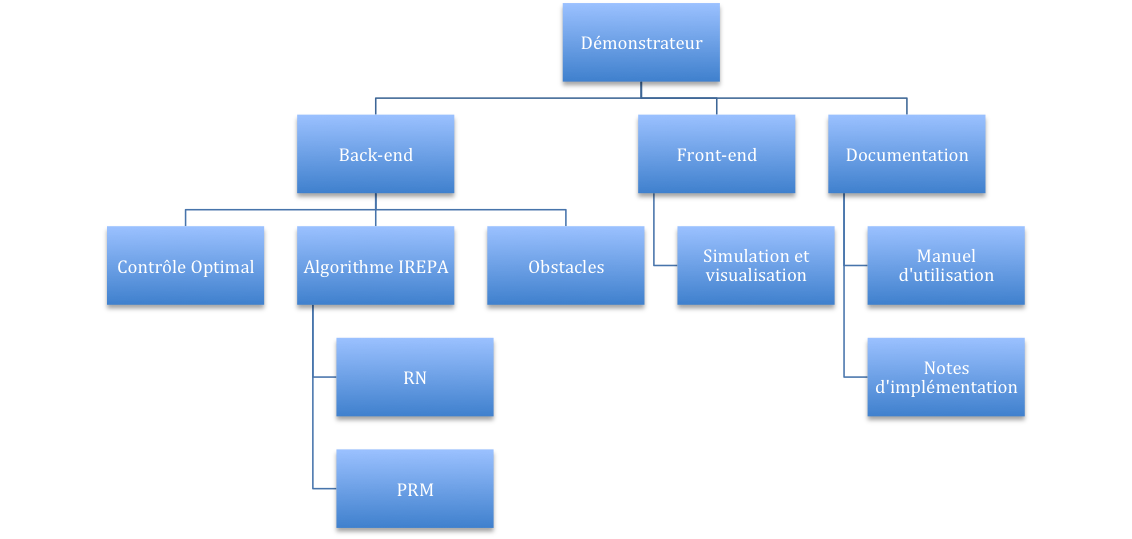
\includegraphics[width=14cm]{pbs.png}
\caption{Diagramme PBS}
\end{figure}


\subsection{Organisation de l'équipe}
Pour pouvoir effectuer le projet, il a été nécessaire d'organiser l'équipe en pôles, autour de tâches spécifiques. Ces attributions ont été faites en fonction des connaissances, souhaits et filières de chacun. Les rôles attribués ont été les suivants : 
\bi
\item Gestion de projet : William Jussiau
\item Algorithme IREPA : Médéric Fourmy \& Guillermo Prieto
\item Contrôle optimal : Martin Renou
\item Simulation-visualisation : Jan Zeman
\ei

Certaines tâches dans des pôles requérant peu d'expertise pourront être effectuées par un membre de l'équipe qui n'est à l'origine pas affecté à ce pôle. 

La répartition des tâches est résumée dans le diagramme RACI joint (légende : A - accountable en orange; R - responsible en jaune; C - consulted en vert; I - informed en bleu).

\begin{figure}[!htb]
\centering
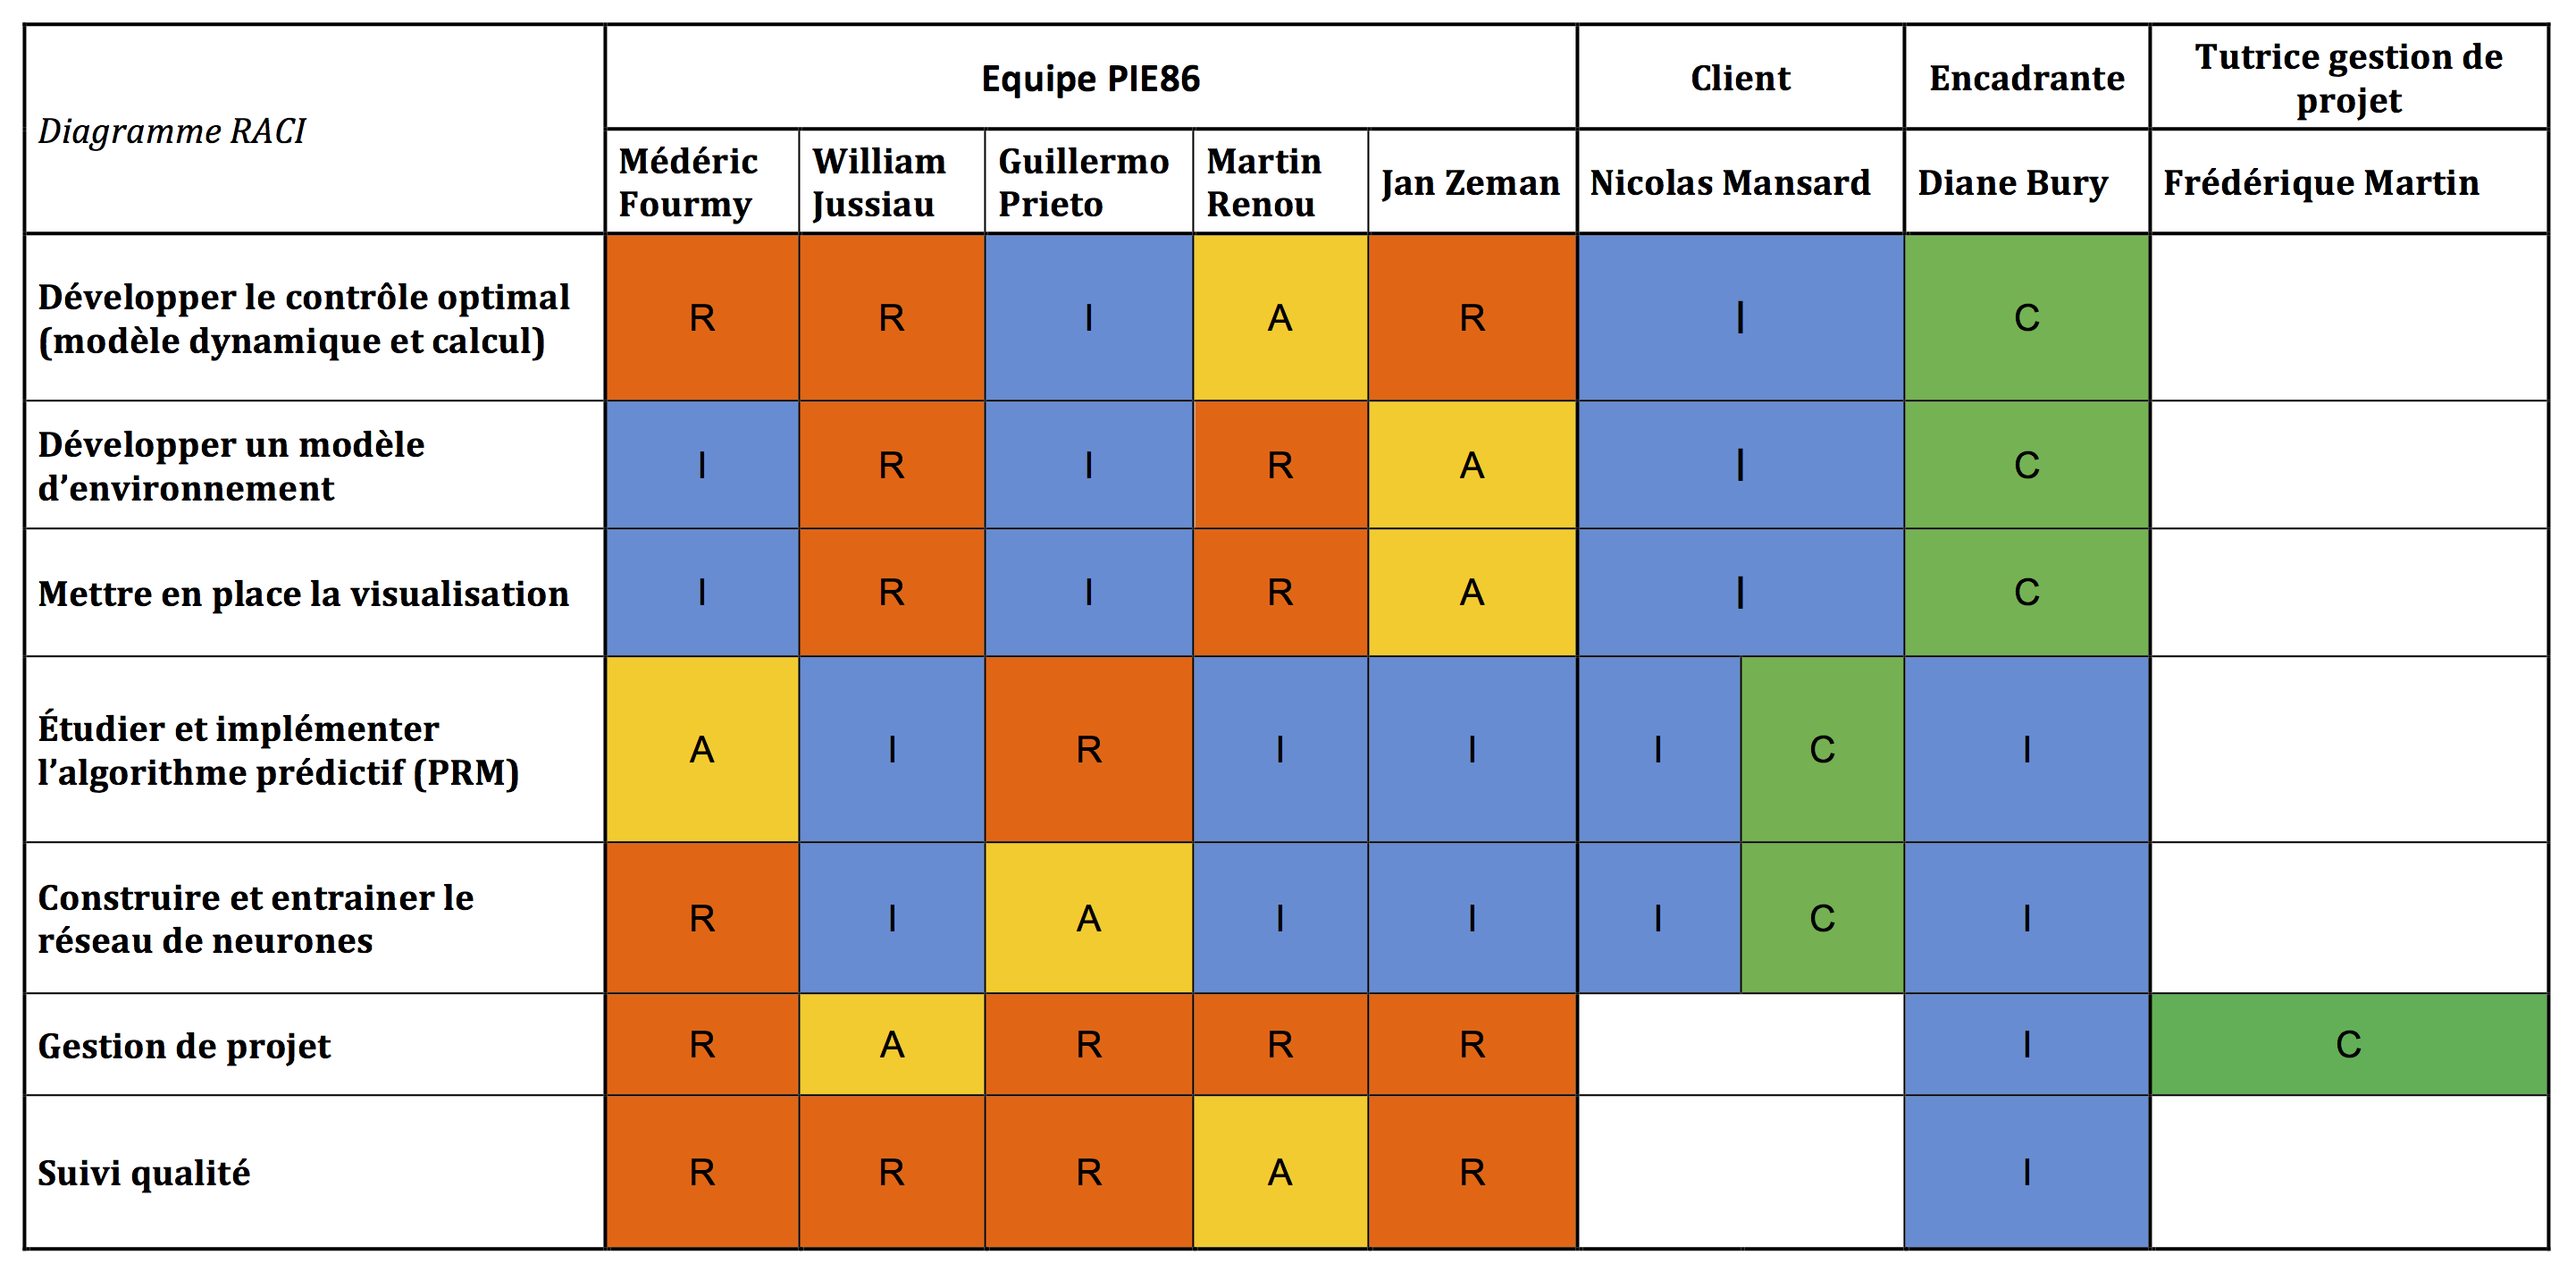
\includegraphics[width=16cm]{RACI.png}
\caption{Diagramme RACI du projet}
\end{figure}

\subsection{Organisation du travail}
\subsubsection{Outils, méthodes}
Cette partie pourra être redondante avec certaines informations présentes plus haut dans le rapport. On y décrit les outils et méthodes utilisés.

\bi
\itemo Outils
	\bi
	\item Git/GitHub pour la gestion des sources,
	\item l'utilitaire Travis \cite{travis} intégré à GitHub, qui ne permet la gestion automatique des normes de codage (en particulier : l'impossibilité pour un développeur de proposer un code non conforme),
	\item Framateam.org (basé sur Mattermost \cite{mattermost}) pour les communications techniques. Il est possible d'y créer des canaux afin de discuter en petit comité, d'y partager des documents, du code, etc. Ont accès à l'outil : les 5 membres du groupe et Diane Bury,
	\item Facebook Messenger pour les communications "projet" internes (ex. réunions), 
	\item e-mailing pour les communications externes (ex. avec Nicolas Mansard ou Frédérique Martin).
	\ei

\itemo Méthodes
	\bi
	\item Gestion des sources : procédé recommandé par les utilisateurs de Git et formalisé par Martin Renou lors de la réunion du 20/12/17. La gestion des sources se fera en langue anglaise : toutes les étiquettes associées à des actions (ex. commentaire d'un \textit{commit} ou d'une \textit{pull request}) devront être rédigées en anglais,
	\item Normes de codage : normes liées au langage (C/C++, bash : GNU Coding Standards \cite{gnu} ; Python : PEP8 \cite{pep8}). Le choix du langage reste à discrétion de l'étudiant, en accord avec les autres membres du groupe si nécessaire,
	\item Rédaction de code : le code est rédigé et commenté en anglais,
	\ei
\ei



\subsubsection{Définition des jalons}
Aucun jalon n'a été explicitement imposé par le client - ont seulement été évoqués des simulateurs prenant en compte différentes complexités (dans le modèle dynamique, l'environnement...). Nous avons ainsi défini au sein de l'équipe, avec l'aval du client, plusieurs complexités possibles :
\bi
\itemo Relativement au modèle dynamique :
	\bi
	\item Modèle point sur grille cartésienne : 
	$X = \begin{bmatrix} x \\ y \end{bmatrix}$, 
	$U = \begin{bmatrix} dx \\ dy \end{bmatrix}$,
	
	\item Modèle unicycle : 
	$X = \begin{bmatrix} x \\ y \\ \theta \end{bmatrix}$, 
	$U = \begin{bmatrix} v \\ \omega \end{bmatrix}$
	
	\item Modèle de voiture à définir exactement (possibilités : angulation des roues et vitesses différentielles en virage, inertie des roues, etc.)
	\ei
	
\itemo Relativement à l'environnement :
	\bi
	\item Circulation sur plan libre,
	\item Circulation avec obstacles fixes (cylindres),
	\item Circulation avec obstacles fixes de forme avancée (polyèdres) \footnote{La circulation avec des obstacles mouvants n'a pour l'instant pas semblé pertinente au vu de l'algorithme utilisé.}.
	\ei

\ei

\bigskip

	On a donc défini les jalons suivants :
	\bi
	\itemo \textsf{J1} : modèle point basique, simulé sur Gazebo avec prise en compte d'obstacles fixes par \textit{Probabilistic RoadMap} (PRM) simple.
	\itemo \textsf{J2} : modèle uni-cycle, simulé sous Gazebo avec algorithme IREPA complet.
	\itemo \textsf{J3} : modèle de voiture (à définir), simulé sous Gazebo avec IREPA complet.
	\ei
	
	Nous avons aussi évoqué un dernier jalon \textsf{J4} dans lequel nous pourrions développer des utilitaires qui montrent le processus de génération de trajectoire avec IREPA : graphes, trajectoires tracée en temps réel au sol, etc. Comme il ne s'agit pas de fonctions demandées, ce jalon est seulement accessoire. Il pourra aussi contenir un nouveau modèle de voiture.


\subsubsection{Logique de développement}
On utilisera pour le développement une approche incrémentale : chaque jalon correspond à une version fonctionnelle du logiciel, implémentant des modèles de plus en plus complets.

Dans la mesure du possible, les jalons sont indépendants. Cependant, chaque tâche d’un lot de travail requiert que la tâche de l’itération précédente (du même lot de travail) ait été effectuée.

Lorsque les tâches correspondant à un jalon ont été effectuées dans chaque lot de travail, on peut procéder à l’intégration (mise en commun), le test et la validation de cette itération.

\subsubsection{Tâches du projet}
À partir des jalons et des lots de travail, nous avons pu déterminer les tâches plus atomiques à réaliser afin de valider les jalons. Les tableaux ci-dessous présentent toutes les tâches à remplir, de deux manières différente : tâches par jalon (Fig. \ref{fig:taches_par_jalon}) ou par lot de travail (Fig. \ref{fig:taches_par_wp}). Ceux-ci sont disponibles dans l'annexe jointe au présent document.

Nous avons aussi formalisé cela sous Microsoft Project avec un diagramme de Gantt (prenant en compte certains liens temporels entre tâches) et l'emploi du temps (le calendrier de travail étant pris en compte). Les sur-utilisations de ressources ont été laissées telles que calculées par le logiciel - cela correspond à du travail supplémentaire à fournir par rapport au calendrier de base.



\subsubsection{Évaluation du temps}
D'après les tâches précédemment mises en avant, nous avons pu évaluer le temps nécessaire à la réalisation du projet. Il a été et sera nécessaire de le réévaluer aussi souvent que possible, en fonction de l'avancement des tâches et d'éventuelles complications.


\begin{figure}[!htb]
\centering
\begin{tabular}{ | p{7.5cm} | p{7.5cm} | }
\hline
Tâches & Temps alloué \\
– Gestion de projet & 100 h \\
– Mise en route & 120 h \\
– Développement & 140 h \\
– Intégration + tests & 75 + 10 h \\
\hline
Réalisation du projet & 445 h \\
\hline
Marge & 80 h \\
\hline
Charge de travail totale & 525 h \\
Charge de travail par personne & 125 h \\
\hline
\end{tabular}
\caption{Évaluation du temps alloué au projet}
\end{figure}




\subsection{Risques identifiés}
Nous avons pu identifier un certain nombre de risques, regroupés dans le tableau \ref{table:risques} ci-joint. Seuls ceux présentant un fort indice de criticité (nous avons choisi les indices supérieurs à $9/16$, correspondant à un score supérieur à 3/4 simultanément en probabilité et gravité) seront sujet à un plan d'action, afin que le projet soit perturbé le moins possible.

\begin{figure}[!htb]
\centering
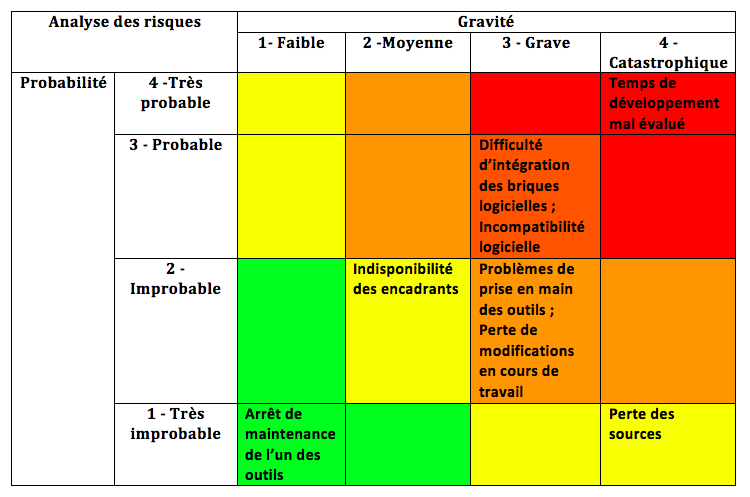
\includegraphics[width=14cm]{risques.png}
\caption{Risques mis en avant}
\label{table:risques}
\end{figure}

Les risques les plus critiques sont décrits dans le tableau \ref{table:risques_importants}.

\begin{figure}[!htb]
\centering
\begin{tabular}{| p{4.5cm} | p{5cm} | p{5cm} |}
\hline
Risque & Cause & Conséquence \\
\hline
\hline
Temps de développement mal évalué & Manque d'expertise et de connaissances du domaine & Blocage projet, retard sur les livrables \\
\hline
Difficulté d'intégration des briques logicielles & Spécifications vagues ou non-respect des spécifications & Retard, modifications à apporter, revue des spécifications \\
\hline
Incompatibilité logicielle & Mauvais référencement des versions ou matériel non adapté aux logiciels & Retard projet ou changement de logiciels utilisés \\
\hline
\end{tabular}
\caption{Risques les plus importantes, leurs causes et conséquences}
\label{table:risques_importants}
\end{figure}


Leur impact sera mitigé de la manière décrite dans le tableau \ref{table:gestion_risques}. Notons que l'action préventive pour le risque d'incompatibilité logicielle (qui consiste à choisir le logiciel en fonction du matériel disponible) n'est pas satisfaisante : nos possibilités seraient bridées. Après beaucoup d'efforts, nous somme parvenus à installer et faire fonctionner tous nos logiciels sur les ordinateurs personnels de tous les membres du groupe.

\begin{figure}[!htb]
\centering
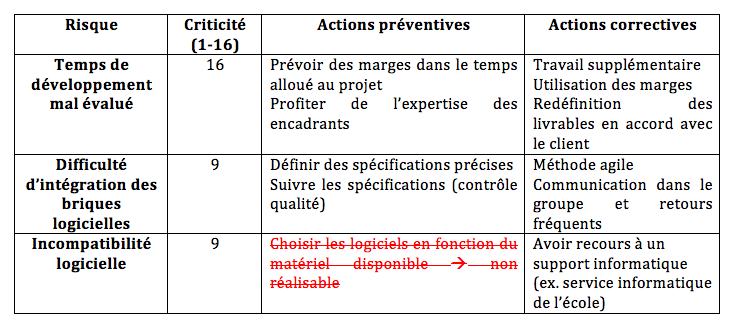
\includegraphics[width=14cm]{gestion_risques.png}
\caption{Gestion des risques les plus critiques}
\label{table:gestion_risques}
\end{figure}
%%%%%%%%%%%%%%%%%%%%%%%%%%%%%%%%%%%%%%%%%%%%%%%%%%%%%%%%%







%%%%%%%%%%%%%%%%%%%%%%%%%%%%%%%%%%%%%%%%%%%%%%%%%%%%%%%%%
%\pagebreak
%\afterpage{\null\newpage}
%\clearpage

\chapter{Développement du démonstrateur}

Dans ce chapitre, on détaille le travail effectué. La présentation a été orientée autour de 4 grands axes, qui sont les suivants :

\bi
\itemo La commande et la génération de trajectoire - contexte, principe et apport de l'algorithme IREPA,
\itemo La modélisation de l'environnement et la simulation avec Gazebo,
\itemo La résolution des problèmes de commande optimale avec l'outil ACADO,
\itemo L'architecture finale du code, l'implémentation sous ROS et les résultats.
\ei




\section{Introduction à la génération de trajectoire}
Dans cette section, on va décrire le contexte dans lequel s'inscrit l'algorithme de génération de trajectoire que nous allons mettre en place.

Comme évoqué à plusieurs reprises dans ce rapport, il s'agit de permettre à une voiture de naviguer de manière autonome dans un environnement présentant des obstacles. On cherchera donc un algorithme de contrôle, global, qui permette d'éviter les collisions, en opposition avec un asservissement plus local. Il ne sera donc pas question ici de correcteur PID ou de commande par retour d'état, pour lesquels l'implémentation de base ne permet pas de formuler des contraintes.

\subsection{Contexte de l'approche}
Pour la commande des systèmes dynamiques complexes dans des environnements accidentés, les approches classiques d'automatique peuvent se révéler insuffisantes. Parmi les techniques qui existent, on peut établir deux groupes distincts d'approches :

\begin{enumerate}
	\item Approches avec modèle (ou \textit{model-based}),
	\item Approches sans modèle (ou \textit{model-free}).
\end{enumerate}

%This paper focuses on the control of complex dynamical systems such as UAVs and legged robots. Classical control approaches are hardly applicable to these systems, which represent thus an open problem for the robotics community. Different techniques exist to control complex dynamical systems, most of which can be labeled either as model based, or as model free.

\subsection{Approches \textit{model-based}}
%Model-based approaches, such as Model Predictive Control (MPC), exploit a model of the system to find the control inputs that drive it towards a desired state. Despite their remarkable capabilities and their wide use in robotics, they are severely limited by the associated computation time, which makes their application to large systems extremely challenging. Moreover, model-based techniques need to face the problem of modeling errors, which negatively affect their performance on real hardware.
Ces approches nécessitent que l'on puisse décrire le système (ou le processus) sous la forme d'équations. Typiquement, il s'agit de pouvoir prédire l'état futur d'un système à partir de son état présent et d'éventuelles entrées contrôlées. Un problème de la sorte pourra souvent être formalisé par une équation d'évolution, dont une forme très basique est la suivante :
$$ \dot X = f(X, U) $$ où $X$ est le vecteur d'état du système et $U$ le vecteur de commande appliqué au système.

Parmi ces approches, on s'intéressera tout particulièrement au contrôle prédictif (ou \textit{Model Predictive Control} (MPC)), une approche dans laquelle le but est de trouver la commande $U$ qui amène le système dans l'état désiré $X^\star$, en anticipant le comportement du système selon son équation d'évolution sur un horizon fini glissant, $T$. Le calcul est réitéré à chaque pas de temps sur un horizon de même longueur (d'où l'adjectif "glissant"). Le procédé est illustré par la figure \ref{fig:mpc}.

\begin{figure}[!htb]
\centering
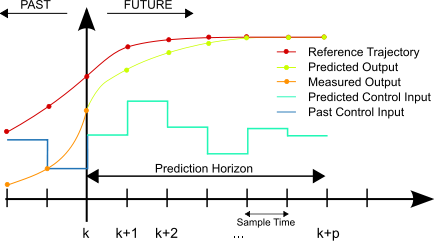
\includegraphics[width=12cm]{mpc_schema.png}
\caption{Illustration du MPC, par Martin Behrendt (licence CC BY-SA 3.0)}
\label{fig:mpc}
\end{figure}



L'un des problèmes qui ressort de cette méthode est une grande sensibilité à la modélisation : une faible erreur de modélisation (dynamique négligée, approximation, etc.) est susceptible d'avoir un impact négatif non négligeable lors du passage sur le système réel. De plus, le temps de calcul d'une telle approche est élevé : c'est une optimisation avec de l'ordre de $T \cdot (n_x + n_u)$ paramètres (pour la version de base, où $n_x, n_u$ sont le nombre d'états et de commandes du système, respectivement), effectuée à chaque pas de temps (fréquence de l'ordre de 10 fois par seconde). Cela rend la technique applicable seulement à des systèmes de faible dimension seulement. De nombreux travaux tentent d'élargir l'approche pour la rendre plus largement applicable \cite{mpc}.



\subsection{Approches \textit{model-free}}
%At the other end of the spectrum we find model- free approaches, such as reinforcement learning [1]. These approaches can learn—either by trial and error or by demonstration—how to control a system to achieve a specified task. 
% Model-free techniques shine exactly where model- based techniques struggle, that is in their computation time and in their adaptation capabilities. However, the off-line learning phase may require unacceptable training times for large systems. Moreover, these techniques need an exhaustive exploration of the state space in order to perform reliably, which in general cannot be ensured.
À l'opposé, les méthodes sans modèle ne nécessitent aucune connaissance a priori sur le système. Parmi les plus connues, on pourra citer l'apprentissage par renforcement, déjà appliqué avec succès au contrôle de systèmes \cite{reinforcement_learning}. Ces approches peuvent apprendre (ex. par essai-erreur) la meilleure commande à appliquer à un système pour effectuer une tâche spécifique. Les avantages de ces techniques sont notamment un coût d'exécution très faible et une robustesse élevée, qui sont exactement les inconvénients des approches avec modèle. Toutefois, elles requièrent souvent un temps d'entraînement (hors-ligne) prohibitif pour des systèmes de dimension élevée, notamment car la plus grande portion possible de l'espace d'état doit être explorée (et cela ne peut jamais être assuré). Par leurs avantages et inconvénients, elles peuvent être vues comme complémentaires des approches précédentes.

\subsection{Complémentarité des approches et algorithme IREPA}
%Given the complementary nature of model-based and model-free approaches, many ways to combine them have been proposed. We can observe two main families of approaches:
%1) Using model-based techniques to speed up the training of model-free techniques.
%2) Learning models/functions to improve the performance of model-based techniques.
Étant donné les caractéristiques des modèles évoquées ci-dessus, nous constatons qu'elles semblent complémentaires. Elles ont été combinées à plusieurs reprises dans des travaux de recherches, de deux manières : 
\begin{enumerate}
%In the first family we can find works from both robotics and computer graphics, where local trajectory optimization has been used to guide the search of a desired control policy [2], [3], [4]. This allows to speed up the training phase (of neural networks in these specific cases) and thus to explore a larger part of the state space. However, this does not completely solve the issue of reliability of the resulting controller, and it needs an extremely accurate learning to avoid unstable control policies.
\item Utilisation de techniques \textit{model-based} pour accélérer l'entraînement de techniques \textit{model-free} \cite{combining_mpc_rl}.

%In the second family we can find different techniques, most of which boil down to learning a certain function off-line, and then using this function on-line inside an MPC. The learned function can be the Value function [5], the system dynamics model [6], or the cost function [7]. The main goal is always to speed-up the MPC computation time and/or to improve the quality of the computed solution. Earlier versions of the same idea consisted in storing a library of optimal trajectories computed off-line, and then use nearest-neighbor to recover the control trajectories to use on-line [8]. The same concept has been applied also to sampling-based planning, where the Value function has been learned to improve the quality of an RRT [9]. Similarly, trajectory optimization has been used to alleviate the curse of dimensionality of dynamic programming [10].
\item Apprentissage de modèles ou fonctions pour augmenter la performance de techniques \textit{model-based}. Par exemple, la fonction approximée peut être utilisée pour initialiser le problème d'optimisation du MPC.
\end{enumerate}


L'algorithme sur lequel nous nous basons est développé dans \cite{mansard} : c'est l'algorithme IREPA\footnote{Dans un souci de concision, on l'évoque par métonymie comme l'algorithme IREPA dans ce rapport (IREPA ne constitue qu'une partie de l'algorithme complet).}. Il exploite les deux familles susmentionnées, à savoir : i) une politique de contrôle est apprise hors-ligne grâce à une méthode avec modèle, et ii) cette politique est ensuite utilisée en ligne pour initialiser le MPC. 

La méthode est détaillée dans la section \ref{sec:IREPA}.




\section{Contrôle optimal et génération de trajectoires}

\subsection{Problème de contrôle optimal}
\subsubsection{Définition}
Pour mettre en oeuvre l'algorithme IREPA, il est nécessaire de résoudre plusieurs problèmes de contrôle optimal. On définit un problème de contrôle optimal comme : 

\begin{center}
\textit{déterminer la commande d'un système qui minimise (ou maximise) un critère de performance, éventuellement sous des contraintes.}
\end{center}

Appliqué à notre système, il s'agira de déterminer la meilleure commande à appliquer à la voiture pour effectuer un trajet, selon son modèle et en évitant des obstacles. Le critère de performance sera traité en suivant.

\subsubsection{Définition formelle}
De façon plus formelle, on définit le problème de la sorte : 

\begin{align*}
    & \arg \min_{X, U}  \hspace{0.5cm} \mathcal{J}(X, U) \\
    & \text{sous les contraintes :} \\
    &  \hspace{1cm} \dot X = f(X,U), \ \forall t \in [0, T] \\
    & 	\hspace{1cm} X \in \mathcal{X} \cap \Omega_{free}, \ \forall t \in [0, T]  \\
    &  \hspace{1cm} X(0) = X_0 \\
    &  \hspace{1cm} X(T) = X_f \\
\end{align*}

Où les termes sont définis de la manière suivante :
\bi
\itemsep1em
\itemo $T$ l'horizon du MPC sur lequel on résout le problème,
\itemo $X, U$ les vecteurs d'état et de commande du système,
\itemo $\dot X = f(X,U)$ l'équation d'évolution du système,
\itemo $\mathcal{J}$ le critère à minimiser. La forme choisie sera discutée plus loin,
\itemo $\mathcal{X} \cap \Omega_{free}$ l'espace des configurations de $X$ qui sont libres (pas d'obstacle),
\itemo $X_0, X_f$ les états de départ et d'arrivée.
\ei

\vspace*{0.5cm}
En bref, les termes de contraintes regroupent le modèle dynamique (qui doit être vérifié à tout temps) et la non-collision avec des obstacles.


\subsubsection{Critère de performance}
Dans l'implémentation de base, on utilisera un critère qui mène à la solution de temps minimal. Cela correspond à $\mathcal{J}(X,U) = \displaystyle \int_{0}^{T} dt = T$. 

On pourra explorer des approches classiques où l'on considère des critères de performance quadratiques :
\vspace{1em}
\bi
\item à énergie minimale : $\mathcal{J}(X,U) = \displaystyle \int U^T R U dt$, où $R$ est une matrice de poids,
\item à état minimal : $\mathcal{J}(X,U) = \displaystyle \int X^T Q X dt$, où $Q$ est une matrice de poids,
\item prenant en compte ces deux contributions : $\mathcal{J}(X,U) = \displaystyle \int U^T R U + X^T Q X dt$.
\ei


\subsubsection{Un outil : ACADO}
Pour résoudre ce problème, on utilise un outil libre développé à la KU Leuven de Bruxelles : ACADO \cite{acado}. Pour citer la présentation que les auteurs font de leur outil, "ACADO Toolkit is a software environment and algorithm collection for automatic control and dynamic optimization. It provides a general framework for using a great variety of algorithms for direct optimal control, including model predictive control, state and parameter estimation and robust optimization". 

À l'aide de cet outil, on sera donc capables de résoudre facilement et efficacement nos problèmes d'optimisation.






\subsection{Méthodes de génération de trajectoires}
\subsubsection{Introduction aux méthodes classiques}

Certaines méthodes classiques de génération de trajectoires visent à déterminer la politique de contrôle optimale. C'est-à-dire, une fonction $\pi^\star : (x, u) \rightarrow x$ qui, à partir d'un état du système, détermine le meilleur contrôle pour amener le système à un nouvel état. 


L'une de ces méthodes classiques se base sur l'utilisation d'une \textit{probabilistic roadmap} (PRM). Dans un premier temps, l'idée est de construire une carte qui relie de façon non-optimale un nombre fini de points, choisis aléatoirement dans l'espace d'état du système. Un chemin entre deux états lointains peut alors être déterminée par un algorithme de type $\mathcal{A}^\star$. Ensuite, cette trajectoire est optimisée par contrôle optimal (solveur \textit{optimal control problem} (OCP) dans ACADO).

La figure \ref{fig:PRM} détaille le fonctionnement de la dite méthode, basée sur une PRM. .


\begin{figure}[!htb]
\centering
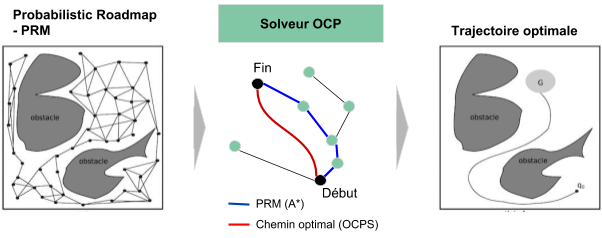
\includegraphics[width=14cm]{image1_1.png}
\caption{Schéma de résolution du probléme de contrôle optimal (OCP) classique utilisant une PRM (\textit{probabilistic roadmap})}
\label{fig:PRM}
\end{figure}



\subsubsection{Méthodes d'approximation de politique de contrôle}

Une extension de cette famille de méthodes consiste à utiliser un estimateur de la politique de contrôle. Il s'agit de construire une fonction de dimension plus faible qui approxime la politique de contrôle. Le plus souvent, le calcul de cet estimateur est long donc effectué hors-ligne, ce qui allège le coût de calcul en ligne. La partie \ref{sec:IREPA} présente l'algorithme utilisé dans ce projet pour établir l'estimateur de politique de contrôle.

La figure \ref{fig:NN} montre le schéma de fonctionnement de cette famille de méthodes. 

\begin{figure}[!htb]
\centering
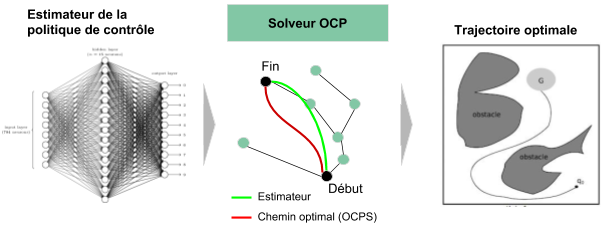
\includegraphics[width=14cm]{image1_2.png}
\caption{Schéma de résolution du problème de contrôle optimal (OCP) utilisant un estimateur de la politique de contrôle optimale}
\label{fig:NN}
\end{figure}

Dans le cadre de ce projet, l'estimateur utilisé est un réseaux de neurones \textit{feed-forward} du type perceptron multi-couches.



\subsubsection{Limitations des méthodes classiques, avantages des méthodes d'approximation}
Bien que relativement efficaces, les méthodes sans approximation souffrent de plusieurs limitations. D'une part, les approches par PRM nécessitent que l'état de départ se trouve dans la PRM, sans quoi on doit chercher l'état de la PRM de le plus proche de l'état courant. D'autre part, elles souffrent d'un important temps de calcul en ligne et sont souvent piégés par des minimum locaux dans l'espace de solutions au problème de contrôle optimal. Les méthodes d'approximation de la politique de contrôle optimale réussissent à surmonter ces difficultés, comme l'explique la figure \ref{fig:limit}.

\begin{figure}[!htb]
\centering
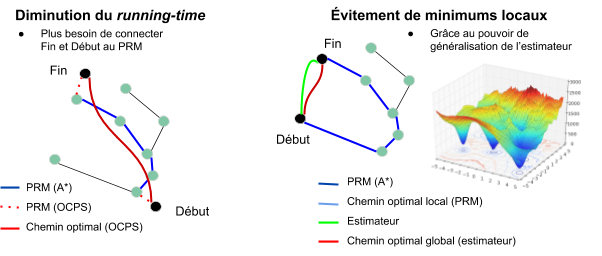
\includegraphics[width=14cm]{image1_3.png}
\caption{Limitations des méthodes classiques de génération de trajectoires}
\label{fig:limit}
\end{figure}


\subsection{Apprentissage de l'approximateur de politique de contrôle : la méthode IREPA}
\label{sec:IREPA}

L'algorithme sur lequel nous nous basons est l'algorithme IREPA, développé dans \cite{mansard}. Son fonctionnement est détaillé dans la figure \ref{fig:IREPA}.

\begin{figure}[!htb]
\centering
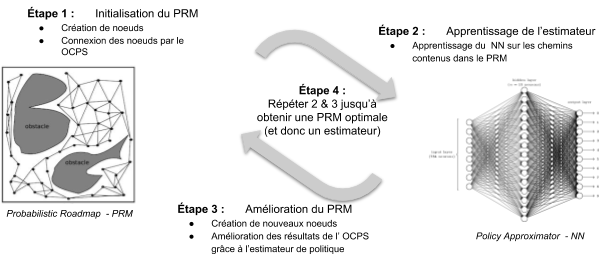
\includegraphics[width=15cm]{image1_4.png}
\caption{Algorithme IREPA d'apprentissage de l'estimateur de la politique de contrôle optimale}
\label{fig:IREPA}
\end{figure}






\subsection{Interaction avec la génération de trajectoire}
L'algorithme IREPA permet donc d'entraîner un réseau de neurones dont la fonction est d'approximer une trajectoire entre deux points donnés. Cette approximation est alors donnée à l'outil de contrôle optimal en tant qu'initialisation d'un problème d'optimisation. Une trajectoire optimisée est finalement retournée en un nombre d'itérations faible.

Le bloc dont le rôle est de réaliser cette tâche (optimisation à partir de l'approximation) est dénommé \textit{Path Finder}. Il prend en entrée deux états à rejoindre (typiquement, des positions dans le plan) ainsi qu'une trajectoire initiale, et retourne une trajectoire optimisée entre ces deux états. En ressources externes, il utilisera le réseau de neurones pour l'initialisation et ACADO pour le contrôle optimal (problème discuté plus loin, dans la section dédiée).

\begin{figure}[!htb]
\centering
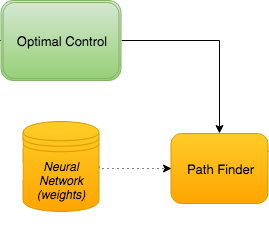
\includegraphics[width=8cm]{pathfinder.png}
\caption{\textit{Path Finder} pour la génération de trajectoire}
\end{figure}





\newpage
\section{Modélisation de l'environnement et simulation}
Les tâches de simulation et visualisation sont prises en charge par un unique logiciel : Gazebo. Nous détaillons plus bas le fonctionnement.

\subsection{Simulation}
Lorsqu'on évoque la simulation, on se réfère à l'étape qui permet de calculer l'évolution d'un système dans un environnement. C'est-à-dire, étant donnés un système commandé (la voiture), un environnement contenant des obstacles et des modèles physiques (gravité, frottements, collision), être capable de prédire l'état du monde dans le futur. Plus formellement, on veut connaître l'état du monde $\mathcal{W}_{k+1}$ à partir d'un état $\mathcal{W}_k$ comprenant le système $\mathcal{S}$, l'environnement $\Omega$ et des modèles physiques $\Phi$ -- ces données étant considérés à l'instant $k$ :
$$ \mathcal{W}_{k+1} = \mathcal{G}( \mathcal{W}_k) = \mathcal{G}(\mathcal{S}_k, \Omega_k, \Phi_k )$$

Dans une première itération, nous avons géré cela manuellement, en développant un simulateur basique. Celui-ci utilisait l'hypothèse que la voiture n'interagissait pas avec l'environnement (pas de collision) et les modèles physiques n'ont pas été nécessaires. En bref, ce premier simulateur nous permettait d'avoir la position suivante de la voiture $X_{k+1}$ à partir de sa position courante $X_k$ et d'une commande $U_k$, tous les autres facteurs étant considérés sans impact sur le comportement du système. Il a ensuite suffi d'afficher la voiture dans son état courant à chaque pas de temps sur Gazebo. Mais Gazebo est plus puissant et peut lui-même simuler un modèle.

Pour la suite, nous avons donc utilisé le moteur de Gazebo \texttt{gzserver}, qui gère tous les modèles nécessaires en plus de celui de la voiture (que nous lui fournissons), en particulier les collisions, la gravité et les frottements. Il suffit de donner à Gazebo tous ces paramètres dans un format spécifique, et on peut ainsi simuler un monde et une voiture.

\begin{figure}[!htb]
\centering
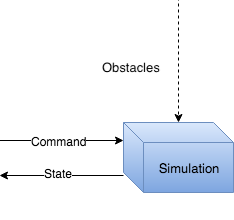
\includegraphics[width=8cm]{simulation.png}
\caption{Simulation avec Gazebo}
\end{figure}




\subsection{Visualisation}
Avec la simulation sous Gazebo s'accompagne un module graphique appelé \texttt{gzclient}, qui permet d'avoir un aperçu du monde simulé. Nous avons donc utilisé cet outil intégré en tant qu'interface graphique pour l'utilisateur.


\subsection{Réalisation de la simulation}
\subsubsection{Modèle de voiture}
La voiture est donnée sous la forme d'un fichier \texttt{urdf} qui est une spécialisation -- propre à Gazebo -- du format \texttt{xml} pour la description de robots.

Un fichier \texttt{urdf} basique contient, en plus du conventionnel nom de modèle, plusieurs sections importantes :

\bi
	\itemo \texttt{visual} : définit le visuel de l'objet, qui sera affiché à l'écran. Pour notre voiture, il a été admis qu'une représentation minimaliste serait suffisante -- il s'agit donc d'un pavé droit. On pourra, dans une version plus avancée, y ajouter des fioritures comme des roues, lui donner une forme plus proche d'une voiture réelle ou ajouter des textures.
	\itemo \texttt{collision} : définit la zone de l'objet qui est sujette à collisions. Dans la plupart des cas (dont le nôtre), il s'agit de l'objet en entier. On pourrait définir un modèle de collision qui englobe légèrement le modèle visuel, afin de préserver ce dernier.
	\itemo \texttt{plugin} : définit la façon dont le modèle interagit avec l'extérieur de Gazebo, notamment comment le mouvement du modèle peut être contrôlé. Cette partie est discutée plus en détails ci-dessous.
\ei


\subsubsection{Contrôle de la voiture : un plugin C++}
Pour contrôler notre modèle de voiture, il est nécessaire de pouvoir faire passer des informations de l'extérieur vers l'intérieur de Gazebo (ex. envoyer une commande à la voiture), et vice-versa (ex. publier l'état actuel de la voiture). Cela permet un contrôle de la voiture en boucle fermée (i.e. la commande envoyée est fonction de l'état actuel de la voiture -- à l'opposé d'une boucle ouverte, où la commande serait envoyée en fonction du temps).

Un plugin doit être codé manuellement, et Gazebo ne propose pas d'outil officiel de support du langage Python, ce qui nous a obligé a coder cette partie en C++. De nombreux tutoriels de Gazebo expliquent la création d'un plugin pour le contrôle d'un modèle, donc cela n'a pas posé de problème majeur. Il est même possible de lier un plugin Gazebo avec des instructions ROS, ce que nous avons fait, pour pouvoir commander la voiture à partir de l'algorithme que nous inclurons dans ROS.



\subsubsection{Obstacles}
Les obstacles sont à l'origine définis par l'utilisateur dans un fichier \texttt{obstacles.obs}  qui a une syntaxe \texttt{xml}. Cela permet à l'utilisateur de préciser chacun des obstacles, cylindriques pour l'instant, sous la forme de trois paramètres : une position et un rayon --- $(x, y, R)$.

Mais cela n'est pas suffisant pour afficher et simuler les obstacles avec Gazebo. Plusieurs étapes intermédiaires doivent être effectuées avant d'obtenir les obstacles dans la simulation : extraire les paramètres de chaque obstacle et créer un modèle \texttt{urdf} propre à chaque obstacle, puis afficher ce modèle dans le monde simulé.

Chaque obstacle ayant une structure de fichier \texttt{urdf} proche (les champs sont les mêmes, seuls les paramètres de taille et placement sont modifiés), nous avons utilisé un utilitaire livré avec ROS : \texttt{xacro} (contraction de "xml" et "macro"). À partir d'un fichier "type" d'obstacle cylindrique (i.e. avec des paramètres formels), il sera possible de définir des fichiers proches dont les paramètres seront choisis.

Pour la prise en compte des obstacles dans le monde simulé, Gazebo offre un service disponible depuis ROS : \texttt{spawn\_model}.

On affichera donc les cylindres avec l'algorithme suivant :

\begin{framed}
Pour chaque obstacle dans le fichier \texttt{obstacles.obs} :
\begin{enumerate}
\itemsep0em
\item Lire les paramètres de l'obstacle, 
\item Exécuter l'utilitaire \texttt{xacro} pour créer le fichier \texttt{urdf} associé, 
\item Générer l'obstacle dans le monde avec \texttt{gazebo\_spawn\_model}.
\end{enumerate}
\end{framed}



\subsubsection{Illustration de la simulation}
On montre ci-dessous l'aspect visuel de la simulation, telle que développée sous Gazebo. Plusieurs éléments apparaissent ici : les cylindres correspondent aux obstacles, la roue représente la voiture, le cône de chantier symbolise le point de départ et le panneau stop, l'arrivée. Ces objets ont été placés de façon arbitraire dans un but d'illustration uniquement.

\begin{figure}[!htb]
\centering
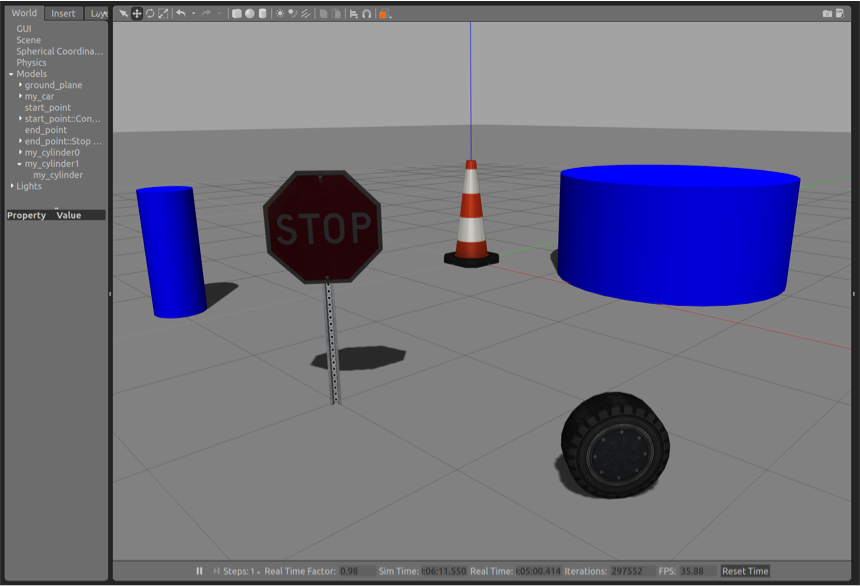
\includegraphics[width=14cm]{gzclient.png}
\caption{Notre simulation sous Gazebo}
\end{figure}








\newpage
\section{Implémentation}
\subsection{Architecture haut niveau}

On illustre notre logiciel par le schéma suivant, qui représente les blocs majeurs de l'implémentation. On représente en rouge le fichier contenant les obstacles, en bleu la simulation, en jaune la génération de trajectoire, et en vert les problématiques liées à la résolution du contrôle optimal.

De plus, on met en avant les deux phases de l'algorithme : à gauche, la partie hors-ligne (construction du réseau de neurones), et à droite, la partie en ligne (génération de trajectoire et simulation).

\begin{figure}[!htb]
\centering
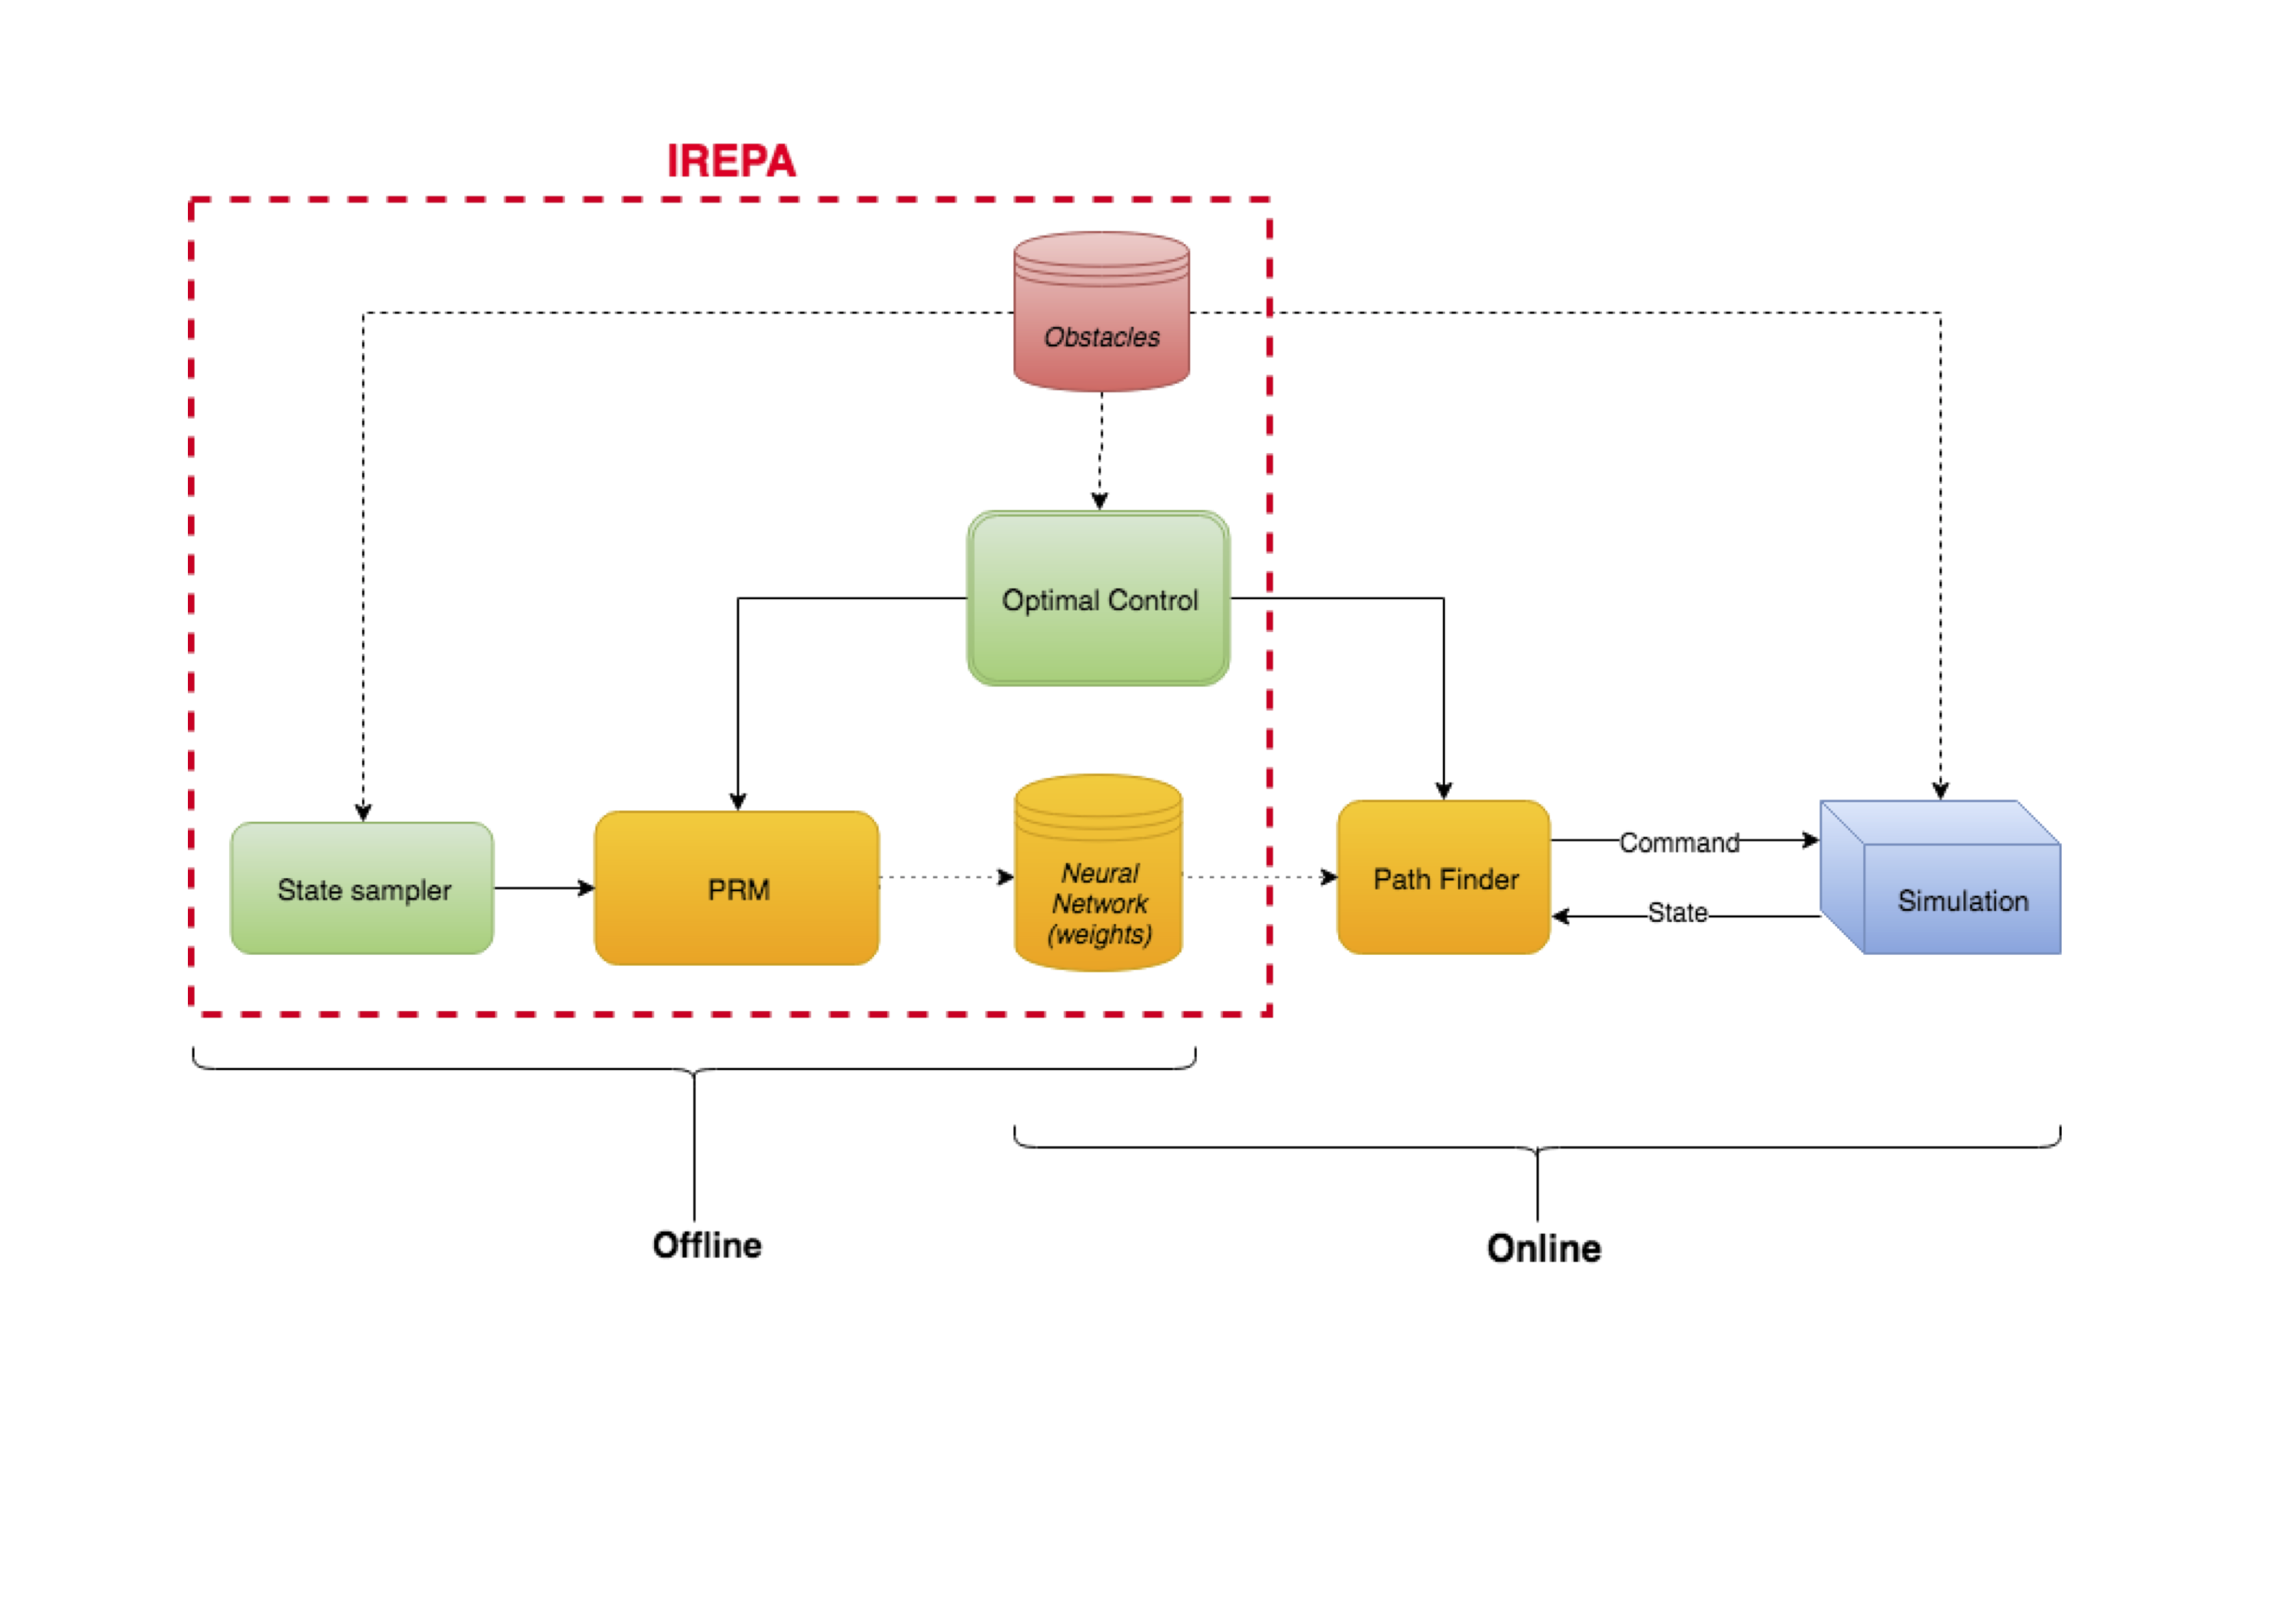
\includegraphics[width=16cm]{architecture_projet.png}
\caption{Architecture haut-niveau du démonstrateur}
\end{figure}



\subsection{Architecture ROS}
ROS est un logiciel qui propose une large gamme de fonctions pour la communication entre différents morceaux de codes, indépendamment du langage utilisé (utile dans notre cas, car nous avons utilisé Python et C++). Il met à notre disposition trois modes de communications que nous utilisons pour des cas de figures distincts :

\bi
\itemo un \texttt{topic} : permet de publier une information sur un canal de communication, à une fréquence donnée. Typiquement, on utilisera des \texttt{topics} pour publier à intervalles de temps donnés la commande pour la voiture, ainsi que publier l'état de la voiture depuis le simulateur. 

\itemo un \texttt{service} : basé sur le schéma client/server. Un premier noeud \textit{client} effectue une requête à un autre noeud sur lequel tourne en continu un \textit{server} de service. Le premier noeud reçoit une réponse synchrone, c'est-à-dire qu'il est bloquant en attendant la réponse. On utilisera les \texttt{services} pour des opérations courtes pouvant se faire de manière synchrone sans ralentir le reste du démonstrateur. On peut par exemple citer la requête permettant de récupérer la liste d'obstacles.

\itemo une \texttt{action} : basée sur les topics, cette surcouche permet des communications asynchrones de type client/server. Un client envoie une requête à un server d'action et peut choisir d'attendre sa réponse où de continuer à effectuer d'autres tâches. Dans les deux cas, il est possible de traiter des informations quant à l'avancement de la tâche demandée pendant son exécution. Ce mode est adaptée aux taches longues comme le calcul du contrôle optimal en ligne.
\ei

\vspace{0.5cm}

\underline{NB} : Il est possible d'obtenir un graph de l'ensemble des topics et services en fonctionnement après avoir lancé une application ROS, en utilisant la commande suivante dans un nouveau terminal : 
\texttt{rosrun rqt\_graph rqt\_graph}.




\subsection{Répertoire et code source}
\subsubsection{Organisation du répertoire}
L'organisation du répertoire des sources a été modifiée à plusieurs reprises pendant le développement. Il est néanmoins possible de noter une constante : dans chaque architecture du répertoire, nous avons séparé en différents dossiers les fonctions indépendantes du logiciel. Par exemple, on forme des dossiers contenant :

\bi
\itemo le contrôle optimal $\rightarrow$ \textit{opt\_control}
\itemo la simulation $\rightarrow$ \textit{display}
\itemo l'algorithme IREPA $\rightarrow$ \textit{roadmap}
\itemo la gestion des obstacles $\rightarrow$ \textit{obstacles}
\itemo les fichiers de lancement $\rightarrow$ \textit{demo\_launch}
\ei


\subsubsection{Code source}
Le code source est disponible sur GitHub, à l'adresse suivante : 

\begin{center}
\texttt{https://github.com/PIE86/MemoryEnhancedPredictiveControl}
\end{center}

Il contient tous les documents nécessaires pour l'installation et la manipulation du logiciel du projet de cette année (2018), ainsi que les projets des années précédentes (2016, 2017).
%%%%%%%%%%%%%%%%%%%%%%%%%%%%%%%%%%%%%%%%%%%%%%%%%%%%%%%%%



\section{Résultats}
Dans cette section, nous présentons les résultats de l'implémentation d'IREPA pour la modélisation simple d'une voiture. Nous nous intéresserons d'abord aux preuves de l'applicabilité de la méthode à ce système, puis aux trajectoires générées par le contrôle optimal et enfin à la question de l'implémentation d'un contrôleur on-line.

\subsection{Construction de la PRM et apprentissage du réseau}

Comme expliqué précédemment, chaque itération d'IREPA se déroule en trois étapes.
\begin{itemize}
	\itemo \textbf{Expansion}: on essaie de connecter l'ensemble des noeuds non connectés de la PRM deux à deux. À l'initialisation (itération 0), l'estimateur n'est pas entraîné. Le contrôleur optimal utilise donc son initialisation par défaut, ou le plus court chemin déjà existant dans le graphe ($\mathcal{A}^\star$).
	\itemo \textbf{Apprentissage}: on entraîne l'estimateur (les réseaux de neurones) en utilisant les arêtes enregistrées dans le graphe.
	\itemo \textbf{Amélioration} : chaque arête pour laquelle on trouve une meilleure estimation avec le réseau de neurone est améliorée en initialisant le contrôle optimal avec cette estimation. Si la trajectoire trouvée n'est pas elle aussi bonne que la trajectoire déjà présente, elle est abandonnée.
\end{itemize}

\vspace{0.5cm}

Une des questions de ce PIE était de savoir si l'algorithme était applicable aux calcul de trajectoire pour une voiture. On peut le vérifier si on parvient à montrer qu'il est possible de construire un estimateur permettant un démarrage à chaud du contrôleur optimal (i.e. un estimateur tel que, lorsque le contrôleur optimal est initialisé avec l'estimation, la trajectoire trouvée est meilleure que sans intiialisation). 

Les figures \ref{fig:attempts} et \ref{fig:connectivity} en sont l'illustration. Sur la première, les courbes bleue, verte et orange sont respectivement le nombre de connections réussies en initialisant avec le plus court chemin ($\mathcal{A}^\star$), l'estimateur et le nombre total d'essais à chaque itération. Le deuxième graphes représente quant à lui l'évolution du nombre de connections à l'issue de chacune des itérations d'IREPA. La ligne en pointillés correspond au nombre maximal de connections possibles ($C=n(n-1)$ où $n$ est le nombre de noeuds).

Ces figures montrent donc que l'estimateur remplit sa tâche : il permet de connecter de plus en plus de noeuds au fur et à mesure de son apprentissage, jusqu'à un graphe quasiment complètement connecté.

\begin{minipage}[b]{0.45\textwidth}
	\begin{center}
	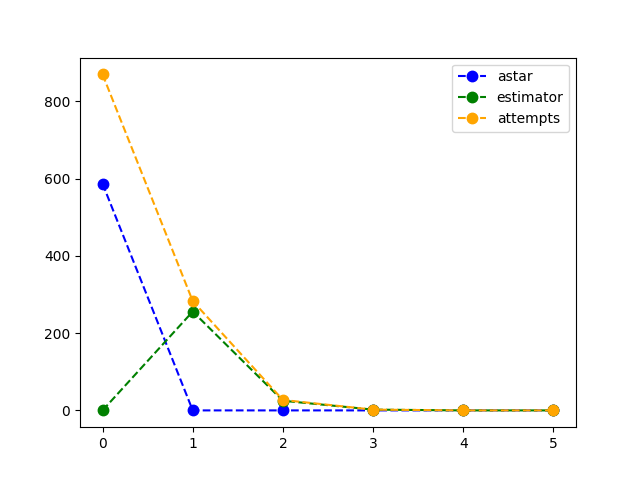
\includegraphics[width=1\linewidth]{images/connect_attempts_30nodes_6iterations.png}
		\captionof{figure}{Nombre de connections effectuées à chaque itération}
		\label{fig:attempts}
	\end{center}
\end{minipage}
\hfill
\begin{minipage}[b]{0.45\textwidth}
	\begin{center}
		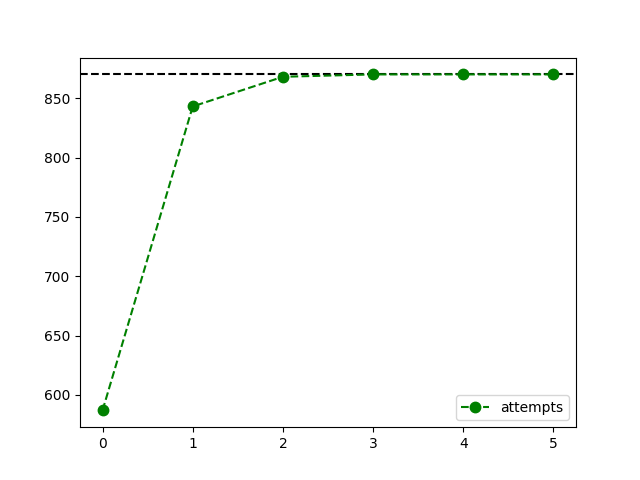
\includegraphics[width=1\linewidth]{images/connectivity_30nodes_6iterations.png}
		\captionof{figure}{Nombre de connections à l'issue de chaque itérations}
		\label{fig:connectivity}
	\end{center}
\end{minipage}
\vspace{0.5cm}

Il est également intéressant d'observer l'évolution du coût total, qui est censé baisser du fait de l'étape d'amélioration. On rappelle que nous avons choisi d'utiliser le temps de la trajectoire comme fonction de coût. Sur la figure \ref{fig:total_edges}, on a en gris le coût total des arêtes du graphe à chaque itération (après l'étape d'expansion) avant amélioration des arêtes, et en vert le coût après améliorations. On observe que les différences de coûts sont très importantes sur les 3 premières itérations et deviennent faibles par la suite.

\vspace{0.5cm}

\begin{center}
	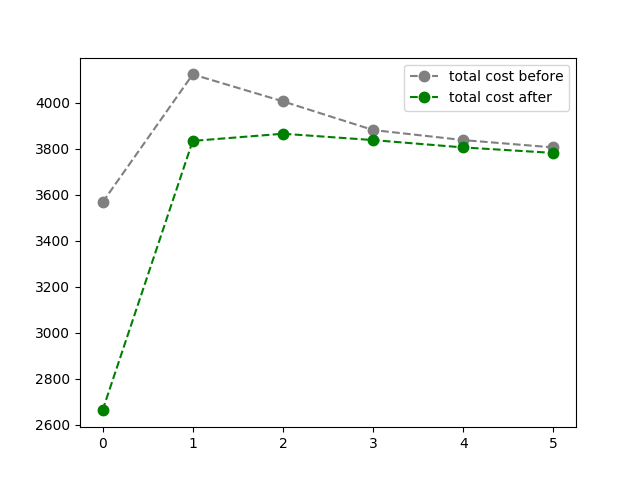
\includegraphics[width=0.48\linewidth]{images/total_edges_cost_30nodes_6iterations.png}
	\captionof{figure}{Coût total des arêtes avant et après amélioration}
	\label{fig:total_edges}
\end{center}


\subsection{Génération de trajectoires}
Après avoir montré que l'apprentissage est possible avec ce modèle, nous allons étudier les trajectoires obtenues par contrôle optimal initialisé avec l'estimateur. Nous avons sélectionné deux trajectoires représentatives de l'apport de l'initialisation avec l'estimateur sur le calcul du contrôle optimal.

\subsubsection{Trajectoire simple}
\begin{itemize}
	\itemo départ: $x=2,\ y=2,\ \theta=0$
	\itemo arrivée: $x=12,\ y=15,\ \theta=0$
\end{itemize}

Cette trajectoire paraît relativement simple à déterminer : elle ne comporte pas de rotation trop importante, n'y d'obstacles à proximité. La figure \ref{fig:traj1_controls} représente les graphes de l'angle $\theta$ (en noir) et des contrôles en vitesses linéaire et angulaire $v$ et $w$ (en bleu), en fonction du temps. Les graphes du dessus correspondent à la trajectoire calculée avec l'initialisation par défaut d'ACADO, et ceux du dessous à celle avec l'initialisation de l'estimateur entraîné. Sur la figure \ref{fig:traj1_2D}, on observe en vu de dessus les différentes trajectoires calculées.

\begin{itemize}
	\itemo En rose: trajectoire calculée par l'estimateur
	\itemo En orange: trajectoire calculée par le contrôle optimale avec initialisation par défaut
	\itemo En bleu clair: trajectoire calculée par le contrôle optimal avec initialisation de l'estimateur
\end{itemize}

Les trajectoires suivent des chemins assez proches en 2D mais le temps de trajet sans initialisation de l'estimateur est de 6.86s contre 2.1s avec. Cela s'explique par le fait que les contrôles sont dans le deuxième cas saturés. Par exemple, pour le contrôle en vitesse angulaire w, on a d'abord une valeur de 1 rad/s correspondant à sa borne supérieure, puis 0 et enfin -1 rad/s, la borne inférieure. La vitesse linéaire et durant tout le long à la borne supérieure 5 m/s.

\begin{minipage}[b]{0.45\textwidth}
		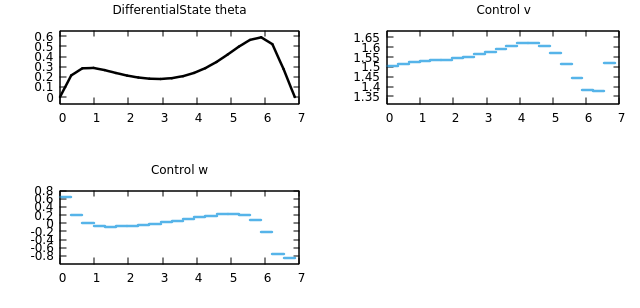
\includegraphics[width=1\linewidth]{images/2_2_0__12_5_0__noinit_trim.png}
		\noindent\makebox[\linewidth]{\rule{\linewidth}{0.2pt}}
		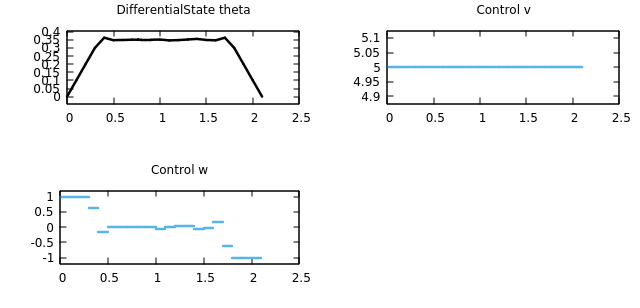
\includegraphics[width=1\linewidth]{images/2_2_0__12_5_0__init_trim.png}
		\captionof{figure}{Angle, contrôle en vitesses linéaire et angulaire en fonction du temps. Haut/bas: sans/avec initialisation de l'estimateur}
		\label{fig:traj1_controls}
\end{minipage}
\hfill
\begin{minipage}[b]{0.45\textwidth}
	\begin{flushright}
		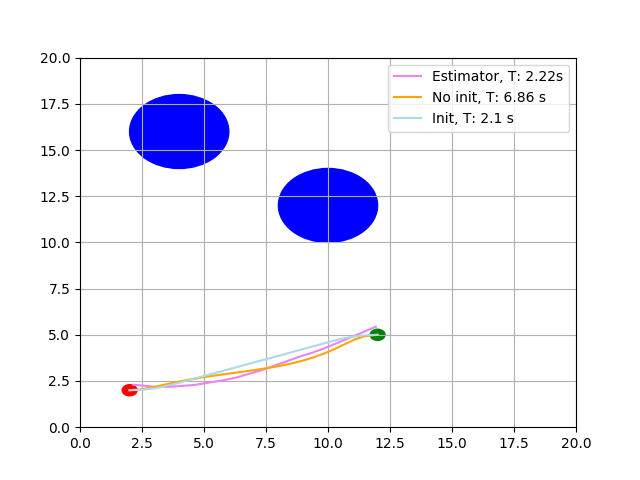
\includegraphics[width=1\linewidth]{images/2_2_0__12_5_0.png}
		\captionof{figure}{Visualisation de la trajectoire et des obstacles. Point rouge/vert: départ/arrivée}
		\label{fig:traj1_2D}
	\end{flushright}
\end{minipage}


\subsubsection{Contournement d'obstacle}
\begin{itemize}
	\itemo depart: $x=7,\ y=1,\ \theta=-1$
	\itemo arrivée: $x=14,\ y=14,\ \theta=1.5$
\end{itemize}
\vspace{0.4cm}

Observons maintenant le cas où la voiture doit contourner un obstacle. Le contrôle optimal sans initialisation donne une mauvaise trajectoire durant de 10.1 contre 2.5s pour la trajectoire bien initialisée. Les deux trajectoire calculées correspondent à des choix différents : dans le premier cas, l'obstacle est contourné par la gauche, la voiture reculant d'abord jusqu'au point d'inflexion, puis allant de l'avant à pleine vitesse, puis reculant encore. Dans le deuxième cas, l'obstacle est contourné par la droite. Encore une fois, on a une saturation des contrôles dans le cas initialisé, notamment la vitesse angulaire qui reste constamment égale à sa borne supérieure 1. \\



{\underline{NB}}: Nous avons choisi de ne pas énumérer un trop grand nombre d'exemples de trajectoires afin de ne pas alourdir ce rapport. On peut cependant évoquer le fait que pour certains calculs non initialisés, le contrôle optimal n'était pas capable de trouver une solution contrairement au cas initialisé. Certains autres résultats ont été présentés lors de la soutenance et sont disponibles dans notre document de présentation.

\begin{minipage}[b]{0.45\textwidth}
	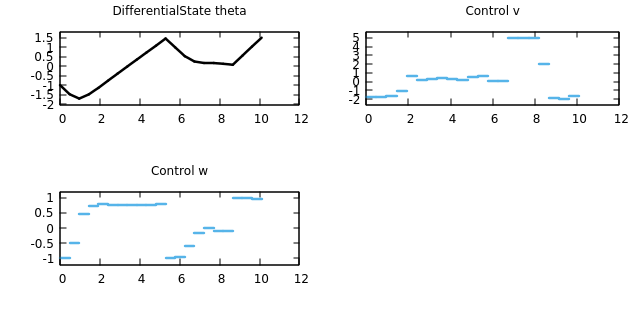
\includegraphics[width=1\linewidth]{images/7_1_-1__14_14_1,5__noinit_trim.png}
	\noindent\makebox[\linewidth]{\rule{\linewidth}{0.2pt}}
	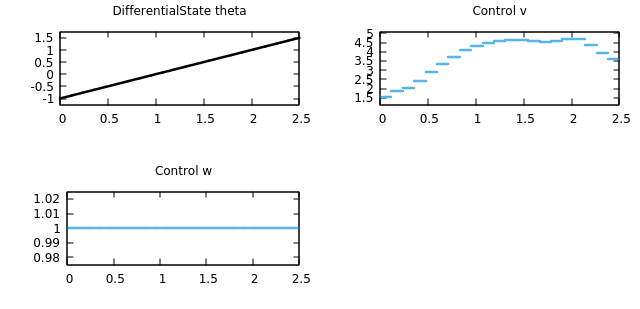
\includegraphics[width=1\linewidth]{images/7_1_-1__14_14_1,5__init_trim.png}
	\captionof{figure}{Angle, contrôle en vitesses linéaire et angulaire en fonction du temps. Haut/bas: sans/avec initialisation de l'estimateur}
	\label{fig:traj2_controls}
\end{minipage}
\hfill
\begin{minipage}[b]{0.45\textwidth}
	\begin{flushright}
		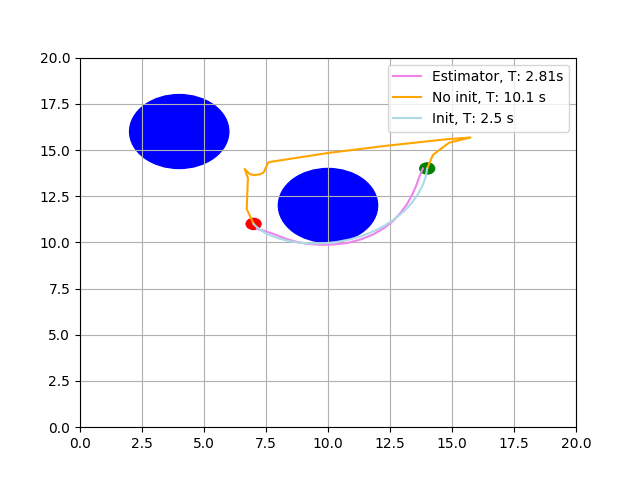
\includegraphics[width=1\linewidth]{images/7_1_-1__14_14_1,5.png}
		\captionof{figure}{Visualisation de la trajectoire et des obstacles. Point rouge/vert: départ/arrivée}
		\label{fig:traj2_2D}
	\end{flushright}
\end{minipage}



\subsection{Contrôle en ligne}
Les trajectoires générées par le contrôle optimal initialisé par l'estimateur semblent donc être optimales et capables d'éviter les obstacles. Théoriquement, il devrait donc être possible d'implémenter un contrôleur online basé sur ces trajectoires. 

Cependant, le facteur temps de calcul est très limitant en ligne, et il nous faut étudier plus en profondeur les possibles relations entre temps de calcul et "difficulté" de la trajectoire. Pour ce faire, calculons les trajectoires partant de $N=400$ points aléatoirement échantillonnés dans l'espace admissible, vers un même point d'arrivée $(x=12,\ y=4,\ \theta=0)$. Pour chacune de ces trajectoires, on récupère la distance euclidienne entre les deux points considérés, le temps de calcul et le temps que dure la trajectoire. On comparera les performances des trajectoires calculées sans et avec initialisation (respectivement à gauche et à droite, à chaque fois).


\paragraph{Temps de calcul et longueur de la trajectoire.}
Un premier graphe intéressant est le tracé du temps de calcul en fonction de la distance euclidienne entre les deux points. On observe que les trajectoires mettent de l'ordre de 0.25s à être calculées avec estimateur, et plutôt 0.10s sans. Il est possible de dégager une légère corrélation positive entre la distance euclidienne et le temps de calcul. Cependant les nombreux cas particuliers et la forte dispersion que l'on observe (calculs entre 0.5s et 2s) rendent difficile l'utilisation de cette métrique comme estimation de la complexité d'une trajectoire.

\begin{minipage}[b]{0.45\textwidth}
	\begin{center}
		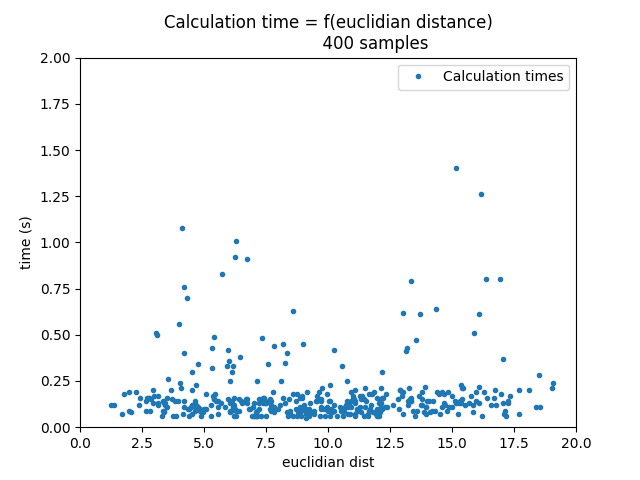
\includegraphics[width=1\linewidth]{images/calc_f(euclid)_noinit.png}
		\captionof{figure}{Temps de calcul en fonction de la  distance euclidienne - sans estimateur.}
		\label{fig:calc_f(euclid)_noinit}
	\end{center}
\end{minipage}
\hfill
\begin{minipage}[b]{0.45\textwidth}
	\begin{center}
		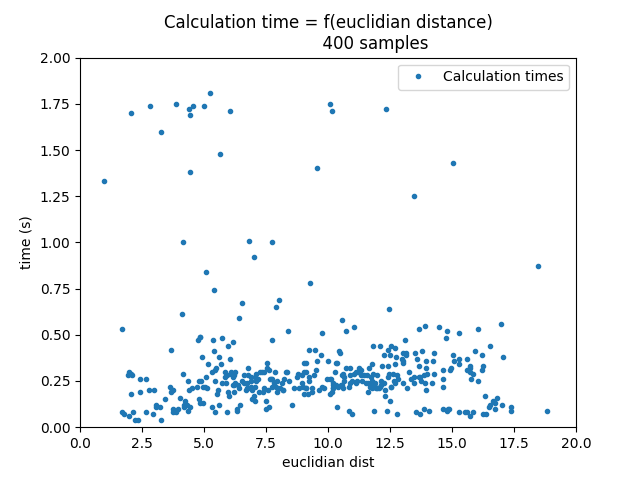
\includegraphics[width=1\linewidth]{images/calc_f(euclid)_init.png}
		\captionof{figure}{Temps de calcul en fonction de la distance euclidienne - avec estimateur.}
		\label{fig:calc_f(euclid)_init}
	\end{center}
\end{minipage}
\vspace{0.5cm}


\paragraph{Temps de calcul et durée de la trajectoire.}
Examinons maintenant la relation entre le temps de calcul et la durée des trajectoires. On n'observe pas de corrélation entre les deux valeurs. Avec estimateur, les trajectoires sont réparties autour d'un même cluster. On note la présence d'un certain nombre de cas particuliers où l'une des valeurs est anormalement élevée et l'autre non.

\vspace{0.5cm}

\begin{minipage}[b]{0.45\textwidth}
	\begin{center}
		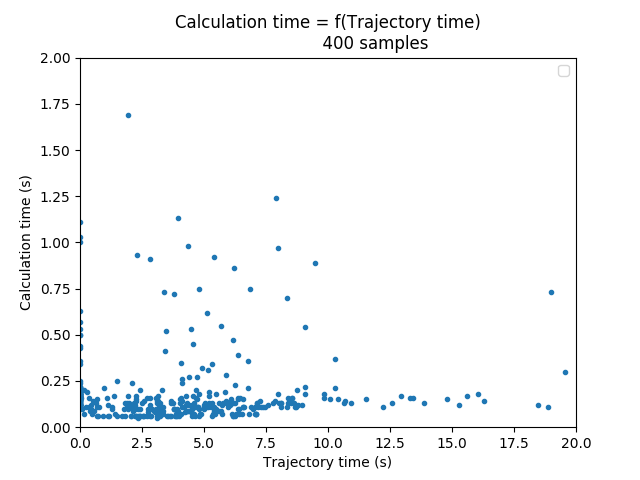
\includegraphics[width=1\linewidth]{images/calc_f(traj)_noinit.png}
		\captionof{figure}{Durée trajectoire en fonction du temps de calcul - sans estimateur}
		\label{fig:calc_f(euclid)_noinit} 
	\end{center}
\end{minipage}
\hfill
\begin{minipage}[b]{0.45\textwidth}
	\begin{center}
		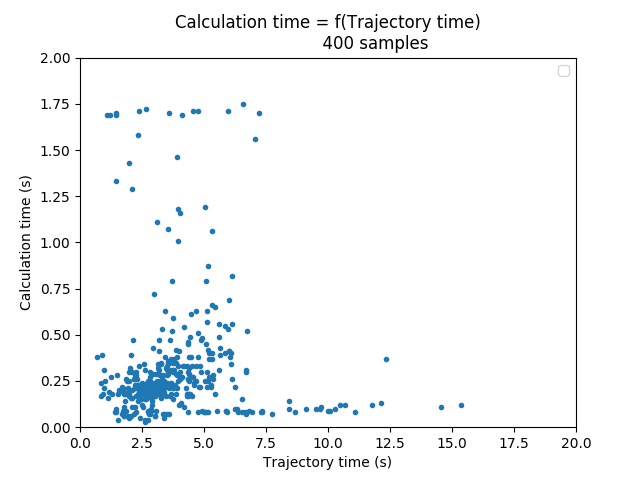
\includegraphics[width=1\linewidth]{images/calc_f(traj)_init.png}
		\captionof{figure}{Durée trajectoire en fonction du temps de calcul - avec estimateur}
		\label{fig:calc_f(euclid)_init}
	\end{center}
\end{minipage}
\vspace{0.5cm}


\paragraph{Longueur de la trajectoire et durée de la trajectoire.}
Enfin examinons la relation entre la distance euclidienne et la durée des trajectoires. On a tracé en bleu les durées des trajectoires et en orange les durées des trajectoires, moins leur temps de calcul. Cette fois, on observe une corrélation positive entre les deux valeurs. On note également de nombreuses valeurs nulles ou négatives pour le cas sans estimateur. Celles-ci correspondent aux cas où le solver n'a pas réussi à converger vers une solution respectant les contraintes du problème. On a aussi certaines valeurs négatives avec l'estimateur, correspondant aux cas où le temps de calcul est supérieur à la durée de la trajectoire calculée. Ces valeurs sont présentes dans le cas où les points sont proches au sens de la distance euclidienne. Ainsi pour les points trop proches, il semble impossible de contrôler le système de cette manière. Une solution pourrait être de se contenter de trajectoire sous optimales pour les points trop proches, de façon à abaisser le temps de calcul nécessaire.


\vspace{0.5cm}

\begin{minipage}[b]{0.45\textwidth}
	\begin{center}
		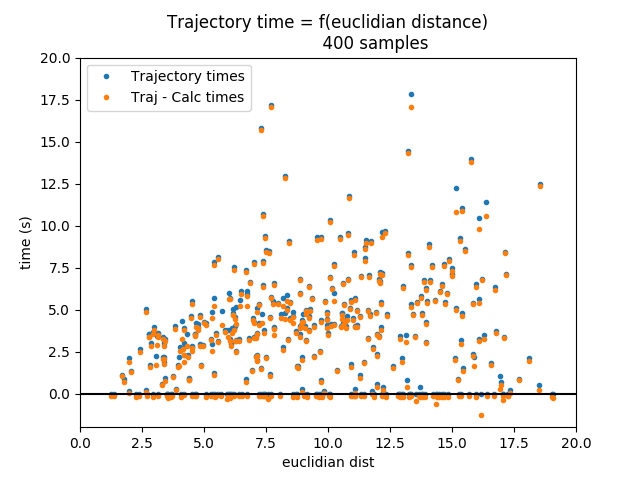
\includegraphics[width=1\linewidth]{images/traj_f(euclid)_noinit.png}
		\captionof{figure}{Temps de calcul = f(Distance euclidienne) - sans estimateur}
		\label{fig:calc_f(euclid)_noinit}
	\end{center}
\end{minipage}
\begin{minipage}[b]{0.45\textwidth}
	\begin{center}
		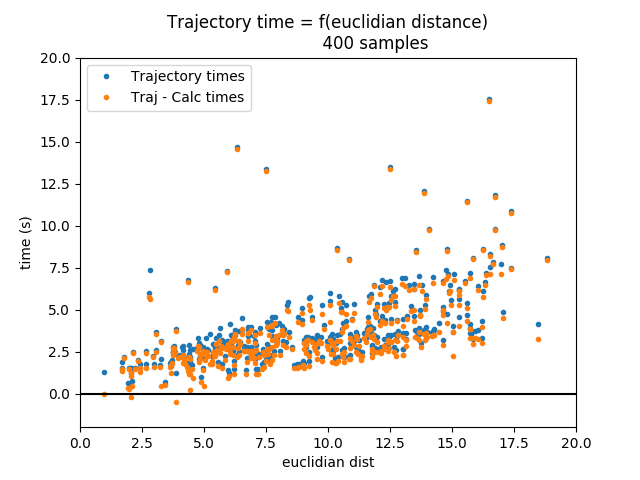
\includegraphics[width=1\linewidth]{images/traj_f(euclid)_init.png}
		\captionof{figure}{Temps de calcul = f(Distance euclidienne) - avec estimateur}
		\label{fig:calc_f(euclid)_init}
	\end{center}
\end{minipage}

\vspace{0.5cm}



La grande incertitude sur le temps de calcul nécessaire à chaque mise à jour de la trajectoire optimale est l'une des difficultés à laquelle nous nous sommes heurtées. Le problème est qu'il est quasiment impossible de prévoir le temps de calcul, et on sait que la voiture aura progressé dans la trajectoire pendant que le contrôleur s'efforce de calculer les nouveaux contrôles... qui ne sont, du coup, plus totalement valables. La principale difficulté que nous avons rencontrée est donc de trouver une fréquence de calcul satisfaisante. Trop grande, le module contrôle optimal reçoit des requêtes de calcul pour de nouvelles trajectoires alors qu'il n'a pas fini de calculer les précédentes -- trop faible, le contrôle sera en retard et de mauvaise qualité.

Nous avons finalement choisi de manière empirique de faire ce calcul à une fréquence de 3Hz.

%%%%%%%%%%%%%%%%%%%%%%%%%%%%%%%%%%%%%%%%%%%%%%%%%%%%%%%%%
\chapter{Conclusion, perspectives}
\section{Synthèse}
Le travail présenté a permis, au travers d'un démonstrateur développer sous ROS et Gazebo, de montrer que l'algorithme IREPA est applicable à la modélisation d'une voiture. On peut notamment mettre en avant les réalisations suivantes : 


\paragraph{Modélisation de l'environnement et simulation à l'aide de Gazebo.} Nous avons pu décrire un environnement (surface plane sur laquelle on trouve des obstacles cylindriques) modulaire, qu'il est possible de simuler avec l'outil Gazebo. C'est dans cet environnement que vit la voiture autonome que nous avons implémentée par la suite. Son contrôle est réalisé à l'aide d'une interaction entre ROS et Gazebo, au travers des plugins C++ proposés par Gazebo.

\paragraph{Contrôle optimal.} Nous avons mis en oeuvre un outil de résolution de problèmes de contrôle optimal : ACADO Toolkit, afin de pouvoir déterminer la \textit{meilleure} trajectoire (dans notre cas : la plus courte) entre deux points de l'espace d'état de la voiture. Ce calcul prend en compte les obstacles présents dans l'environnement.

\paragraph{Approche IREPA.} Enfin, nous avons développé du code réalisant un contrôle grâce à l'approche IREPA, développée au LAAS. Et on a montré la pertinence de cette approche dans le cas de la voiture. En effet, l'apprentissage de l'estimateur permet d'améliorer la PRM en rendant possible la création de nouvelles connexions, et en diminuant le coût de celles existantes. Nous avons pu vérifier que les trajectoires obtenues était satisfaisantes et étaient bien optimales en temps, contrairement à celles obtenues sans initialisation. La fonction de coût temps entraîne des contrôles brusques pour lesquels les commandes sont la plupart du temps saturées.

\paragraph{Gestion de projet.} Nous avons pu, au travers de ce travail, avoir une première vision de la gestion de projet telle qu'elle peut être appliquée dans un contexte industriel. Ce projet étant quasiment purement orienté développement logiciel, nous n'avons pas appliqué toutes les notions de gestion de projet vues en cours, mais celles que nous avons utilisées nous ont bien guidé et ont permis de faire avancer le projet tout au long de l'année. 





\section{Extensions possibles}
On donne ici des pistes pour d'éventuelles extensions et améliorations qu'il serait intéressant d'étudier, dans le cas où le projet devait être repris. Elles sont données dans un ordre arbitraire.

\paragraph{Interface interactive.} 
On pourrait imaginer implémenter des fonctions qui rendent la manipulation du démonstrateur plus agréable pour l'utilisateur : clics pour définir les points de départ et d'arrivée, visualisation des trajectoires calculées, etc.

\paragraph{Obstacles mouvants.} Nous nous sommes limités à des obstacles fixes : il faudrait maintenant étendre la méthode à des obstacles mouvants. Plusieurs solutions semblent possibles, parmi lesquelles nous proposons : utiliser pour les obstacles des paramètres relatifs à la voiture et mesurés à tout temps (ex. par Lidar : angle et distance), ajouter ces paramètres dans l'état de manière dynamique (selon les obstacles visibles). Éventuellement, ajouter une prédiction de la dynamique des obstacles.

\paragraph{Capteurs et simulation réaliste.} Une hypothèse forte de notre projet étaient la connaissance exacte de l'environnement de la voiture (obstacles, dimensions...). Il faudrait maintenant étendre cet algorithme en utilisant un point de vue plus réaliste : en utilisant les données de capteurs, bruitées par exemple, comme seules informations sur l'environnement.

\paragraph{Modèle de voiture complet.} Ce point comprend deux éléments, qui sont : d'une part, l'implémentation d'un modèle complet de voiture dans le calcul optimal (sous forme d'équations différentielles) ; d'autres part, l'implémentation d'un modèle visuel de voiture dans la simulation.

\paragraph{Fonction coût dans le contrôle optimal.} La fonction de coût temps minimal donne des trajectoires brusques. Il pourrait être intéressant d'explorer d'autres fonctions, minimisant par exemple les à-coups (de la commande et/ou des états : ajout des dérivées successives dans la fonction coût), voire une fonction multi-critères.

\paragraph{IREPA.} On pourra, sous la direction de Nicolas Mansard, tenter d'améliorer l'approche IREPA de plusieurs façons : utiliser un même réseau de neurones pour estimer états, contrôles et fonction coût, ajuster les hyper-paramètres du modèle (structure des réseaux), etc.

\paragraph{Contrôleur en ligne.}
Le contrôleur implémenté pour la voiture n'est pas tout à fait satisfaisant -- probablement en partie à cause de la fonction coût utilisée, qui rend le contrôle peu stable. En effet, le calcul de la trajectoire de contrôle étant long à exécuter par rapport à la cadence de contrôle de la voiture, apparaît une contrainte de synchronisation : le calcul du contrôle est lancé lorsque la voiture est à une position donnée, mais se finit lorsque la voiture est à une position suivante -- il n'est donc plus entièrement valable. Il serait intéressant d'étudier plus en détails ce mécanisme, et d'implémenter un contrôleur en ligne robuste et efficace. 



%%%%%%%%%%%%%%%%%%%%%%%%%%%%%%%%%%%%%%%%%%%%%%%%%%%%%%%%%
\newpage
\begin{small}
	\bibliographystyle{unsrt}
	\bibliography{rapport}
\end{small}
%%%%%%%%%%%%%%%%%%%%%%%%%%%%%%%%%%%%%%%%%%%%%%%%%%%%%%%%%


%%%%%%%%%%%%%%%%%%%%%%%%%%%%%%%%%%%%%%%%%%%%%%%%%%%%%%%%%
\newpage
\chapter*{Glossaire des sigles et acronymes}
\addcontentsline{toc}{chapter}{Glossaire des sigles et acronymes}

\begin{tabular}{ >{\bfseries}l  >{\itshape}l  }
PIE & Projet Ingénierie et Entrepreneuriat \\
ROS & Robot Operating System \\
IREPA & Iterative Roadmap Extension and Policy Approximation \\
GUI & Graphical User Interface \\
WBS & Work Breakdown Structure \\
PBS & Product Breakdown Structure \\
MPC & Model Predictive Control \\
PRM & Probabilistic RoadMap \\
RN & Réseau de Neurones \\
OCP(S) & Optimal Control Problem (Solver) \\

\end{tabular}

%%%%%%%%%%%%%%%%%%%%%%%%%%%%%%%%%%%%%%%%%%%%%%%%%%%%%%%%%



%%%%%%%%%%%%%%%%%%%%%%%%%%%%%%%%%%%%%%%%%%%%%%%%%%%%%%%%%
\newpage
\appendix

\chapter{Tableaux des tâches}
Comme évoqué à la fin du chapitre de gestion de projet, on propose ici deux tableaux récapitulant les tâches liées au projet. On les présente sous la forme de deux tableaux : l'un présentant les tâches par jalon (\ref{fig:taches_par_jalon}) et l'autre les présentant par lot de travail (\ref{fig:taches_par_wp}).

\begin{sidewaysfigure}[!htb]
\centering
\makebox[\textwidth][c]{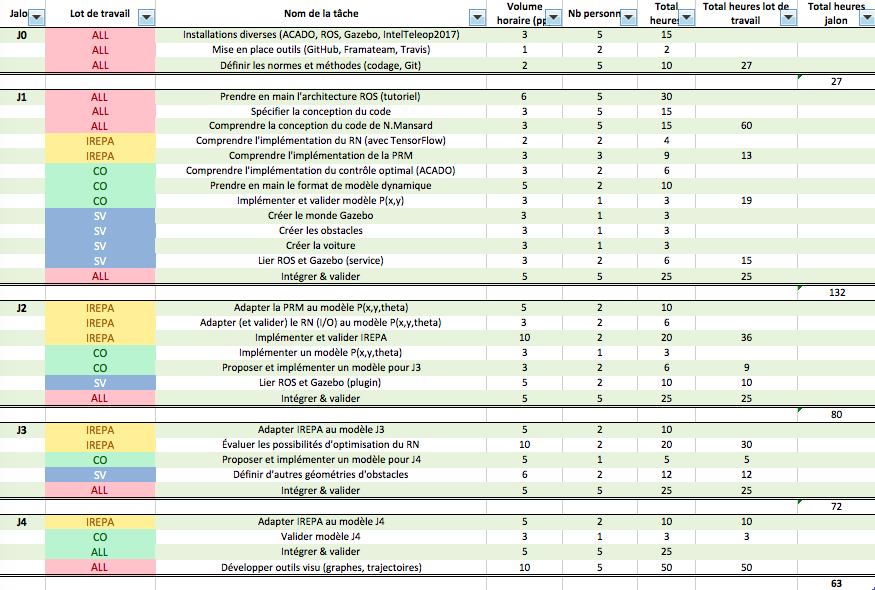
\includegraphics[width=24cm]{jalons.png}}
\caption{Tâches par jalon}
\label{fig:taches_par_jalon}
\end{sidewaysfigure}



\begin{sidewaysfigure}[!htb]
\centering
\makebox[\textwidth][c]{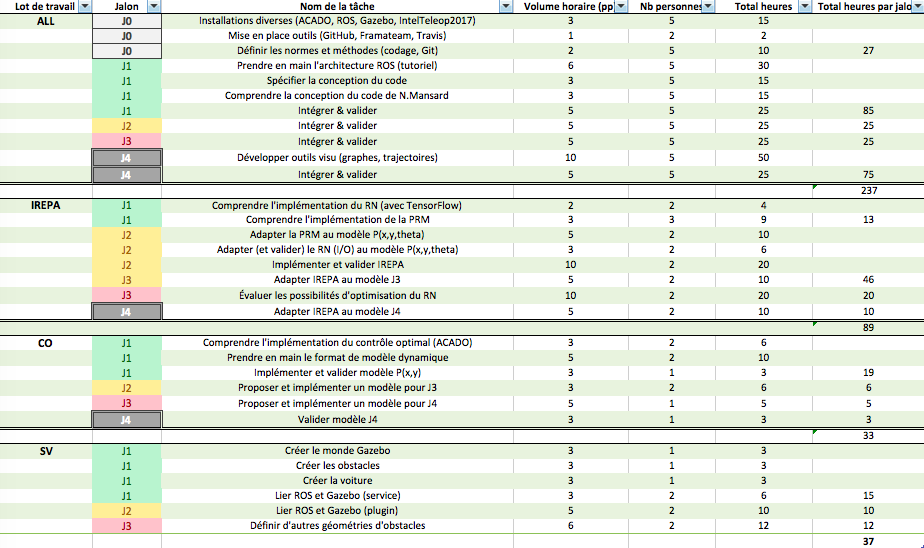
\includegraphics[width=24cm]{wp.png}}
\caption{Tâches par lot de travail}
\label{fig:taches_par_wp}
\end{sidewaysfigure}


%%%%%%%%%%%%%%%%%%%%%%%%%%%%%%%%%%%%%%%%%%%%%%%%%%%%%%%%%




\end{document}














